\documentclass[english,t]{beamer}
%\documentclass[handout,english]{beamer}

\mode<presentation>
{
  \usetheme{Copenhagen}
  % oder ...
  
%  \setbeamercovered{transparent}
  % oder auch nicht
}

%\usepackage[pdftex]{graphicx}
\graphicspath{{/home/ave/doc/images/}{}{../teranaloppu/}{../metodi/}{../slides/Hartikainen/}{../gphealth/}{../2008_09_RSS2008/}{../gphealth/}{../jyvaskyla2009/}{../nbbc2009/}{../gphealth/hippics/}{../euroheis2010/}{../pubgensens2011/}{../reykjavik2013/}{../liverpool2013/}{../../gpstuff/doc/}{./images/}{../aalto_stochastic/}{figs/}{../Stancon2018Helsinki/figs/}{../../paper/cvapprox/}{../gppa2017/}{../valencia2017/}{../../paper/combine_predictive_distribution/tex/}{../venice2018/figs/}{./figs/}}
\usepackage[T1]{fontenc}
\usepackage[utf8]{inputenc}
\usepackage{times}
\usepackage{amsmath,amsfonts,amssymb}
%\usepackage{euscript}
\usepackage{afterpage}
%\usepackage{picinpar}
%\usepackage{array,longtable}
\usepackage{url}
\urlstyle{same}
%\usepackage{eufrak}
\usepackage{amsbsy}
\usepackage{eucal}
\usepackage{rotating}
\usepackage{bm}
\usepackage{pdfpages}
\usepackage{algorithm}
\usepackage[noend]{algpseudocode}
\usepackage{booktabs}
\usepackage{listings}
\usepackage{lstbayes}
\usepackage{microtype}

\usepackage{natbib}
\bibliographystyle{apalike}

\hypersetup{%
  bookmarksopen=true,
  bookmarksnumbered=true,
  pdftitle={Stan},
  pdfsubject={Bayesian data analysis},
  pdfauthor={Aki Vehtari},
  pdfkeywords={},
  pdfstartview={FitH -32768},
  colorlinks=true,
  linkcolor=navyblue,
  citecolor=navyblue,
  filecolor=navyblue,
  urlcolor=navyblue
}

%%%%%%%%%%%%%%%%%%% for tikz figures %%%%%%%%%%%%%%%%%%%%%%%%%%
\usepackage{ifthen}
\usepackage{tikz,pgfplots}
\usetikzlibrary{matrix}
\usetikzlibrary{calc}
\newlength{\figurewidth}
\newlength{\figureheight}


\def\figpdfdir{../venice2018/fig/} % directory for pdf-figures
\def\figtikzdir{../venice2018/tikz/} % directory for tikz-figures 

% this is replacement for the \input command used in the figure-environment which
% takes into account whether pdf is forced
\newcommand{\minput}[2][]{
\ifthenelse{\equal{#1}{pdf}}
	{ \includegraphics{\figpdfdir #2} }
	{ \tikzset{external/remake next} \tikzsetnextfilename{#2} \input{\figtikzdir #2} }
}

% for externalization
\usetikzlibrary{external}
\tikzexternalize[prefix=\figpdfdir] 
\tikzset{external/system call={lualatex
	\tikzexternalcheckshellescape -halt-on-error -interaction=batchmode
	-jobname "\image" "\texsource"}}
    
%%%%%%%%%%%%%%%%%%% for hiding figures %%%%%%%%%%%%%%%%%%%%%%%%%%
\usepackage{color}
\newcommand{\hide}[5][white]{
	% usage: \hhide[color]{vspace,hspace,height,width}
	% note: all measures are relative units measured in \textwidth
	%\begin{minipage}{0.99\textwidth}
	\vspace{#2\textwidth}
	\hspace{#3\textwidth}
	\textcolor{#1}{  \rule{#5\textwidth}{#4\textwidth}  }
	% \end{minipage}
      }

\DeclareMathOperator{\Kfu}{\mathbf{K}_{f,u}}
\DeclareMathOperator{\Kuf}{\mathbf{K}_{u,f}}
\DeclareMathOperator{\Kff}{\mathbf{K}_{f,f}}
\DeclareMathOperator{\iKff}{\mathbf{K}_{f,f}^{-1}}
\DeclareMathOperator{\Kfa}{\mathbf{K}_{f,\tilde{f}}}
\DeclareMathOperator{\Kaf}{\mathbf{K}_{\tilde{f},f}}
\DeclareMathOperator{\Kaa}{\mathbf{K}_{\tilde{f},\tilde{f}}}
\DeclareMathOperator{\Kuu}{\mathbf{K}_{u,u}}
\DeclareMathOperator{\iKuu}{\mathbf{K}_{u,u}^{-1}}
\DeclareMathOperator{\Kau}{\mathbf{K}_{\tilde{f},u}}
\DeclareMathOperator{\Kua}{\mathbf{K}_{u,\tilde{f}}}
\DeclareMathOperator{\Qff}{\mathbf{Q}_{f,f}}
\DeclareMathOperator{\Qaa}{\mathbf{Q}_{\tilde{f},\tilde{f}}}
\DeclareMathOperator{\Qfa}{\mathbf{Q}_{f,\tilde{f}}}
\DeclareMathOperator{\Qaf}{\mathbf{Q}_{\tilde{f},f}}
\DeclareMathOperator{\x}{\mathbf{x}}
\DeclareMathOperator{\f}{\mathbf{f}}
\DeclareMathOperator{\y}{\mathbf{y}}
\DeclareMathOperator{\h}{\mathbf{h}}
\DeclareMathOperator{\uu}{\mathbf{u}}
\DeclareMathOperator{\LL}{\mathbf{\Lambda}}
\DeclareMathOperator{\bb}{\mathbf{b}}
\DeclareMathOperator{\E}{\mathrm{E}}
\def\WAIC{\mathrm{WAIC}}

\newcommand{\kin}{k^{\rm in}}
\newcommand{\kout}{k^{\rm out}}
\newcommand{\gi}{{R_0}}
\newcommand{\eff}{{E_{\rm max}}}
\newcommand{\HN}{{\rm N^+}}
\newcommand{\lN}{{\rm LN}}
\newcommand{\Rss}{R^{\rm ss}}
\newcommand{\invlogit}{\mbox{logit}^{-1}}

% \DeclareMathOperator{\Poisson}{Poisson}
\DeclareMathOperator{\Chi}{Chi}
\DeclareMathOperator{\GP}{\mathcal{GP}}
%\DeclareMathOperator{\N}{N}
\DeclareMathOperator{\KL}{KL}

\DeclareMathOperator*{\argmax}{arg\,max}
\DeclareMathOperator*{\argmin}{arg\,min}
\newcommand{\mb}{\mathbf}
\newcommand{\pkg}[1]{{\fontseries{b}\selectfont #1}}
\newcommand{\proglang}{}
\newcommand{\email}[1]{\href{mailto:#1}{\normalfont\texttt{#1}}}
\newcommand{\doi}[1]{\href{http://dx.doi.org/#1}{\normalfont\texttt{doi:#1}}}
\newcommand{\code}[1]{{\normalfont\texttt{#1}}}

% \DeclareMathOperator{\E}{E}
% \DeclareMathOperator{\VAR}{Var}
% \DeclareMathOperator{\COV}{Cov}
% \DeclareMathOperator{\Prob}{P}
% \DeclareMathOperator{\E}{E}
\DeclareMathOperator{\Var}{Var}
\DeclareMathOperator{\var}{var}
\DeclareMathOperator{\cov}{cov}
\DeclareMathOperator{\logistic}{logistic}
\DeclareMathOperator{\softmax}{softmax}
\DeclareMathOperator{\Multinomial}{Multinomial}
\DeclareMathOperator{\Sd}{Sd}
\DeclareMathOperator{\sd}{sd}
\DeclareMathOperator{\Bin}{Bin}
\DeclareMathOperator{\Poisson}{Poisson}
\DeclareMathOperator{\Beta}{Beta}
\DeclareMathOperator{\logit}{logit}
\DeclareMathOperator{\N}{N}
\DeclareMathOperator{\U}{U}
\DeclareMathOperator{\BF}{BF}
%\DeclareMathOperator{\Pr}{Pr}
\def\euro{{\footnotesize \EUR\, }}
\DeclareMathOperator{\rep}{\mathrm{rep}}

\definecolor{set11}{HTML}{E41A1C}
\definecolor{set12}{HTML}{377EB8}
\definecolor{greenish}{rgb}{0.1333,0.8666,0.1333}
\definecolor{forestgreen}{rgb}{0.1333,0.5451,0.1333}
\definecolor{hutblue}{rgb}{0,0.2549,0.6784}
\definecolor{midnightblue}{rgb}{0.0977,0.0977,0.4375}
\definecolor{navyblue}{rgb}{0,0,0.5}
\definecolor{hutsilver}{rgb}{0.4863,0.4784,0.4784}
\definecolor{lightgray}{rgb}{0.95,0.95,0.95}
\definecolor{section}{rgb}{0,0.2549,0.6784}
\definecolor{list1}{rgb}{0,0.2549,0.6784}
\renewcommand{\emph}[1]{\textcolor{navyblue}{#1}}

%\graphicspath{./pics}

\pdfinfo{
  /Title      (Bayesian data analysis ch7)
  /Author     (Aki Vehtari) %
  /Keywords   (Bayesian probability theory, Bayesian inference, Bayesian data analysis)
}

\parindent=0pt
\parskip=8pt
\tolerance=9000
\abovedisplayshortskip=0pt

%\renewcommand{\itemsep}{0pt}
% Lists
\newenvironment{list1}{
   \begin{list}{$\color{list1}\bullet$}{\itemsep=6pt}}{
  \end{list}}
\newenvironment{list1s}{
  \begin{list}{$\includegraphics[width=5pt]{logo.eps}$}{\itemsep=6pt}}{
  \end{list}}
\newenvironment{list2}{
  \begin{list}{-}{\baselineskip=12pt\itemsep=2pt}}{
  \end{list}}
\newenvironment{list3}{
  \begin{list}{$\cdot$}{\baselineskip=15pt}}{
  \end{list}}

\setbeamertemplate{navigation symbols}{}
\setbeamertemplate{headline}[default]{}
\setbeamertemplate{headline}[text line]{\insertsection}
\setbeamertemplate{footline}[frame number]


\title[]{Bayesian data analysis}
\subtitle{}

\author{Aki Vehtari}

\institute[Aalto]{}
 
\date[]{}

%\beamerdefaultoverlayspecification{<+->}

\begin{document}

\begin{frame}
  
   {\Large\color{navyblue} Chapter 7}

   \begin{list1}
   \item 7.1 Measures of predictive accuracy
   \item 7.2 Information criteria and cross-validation
     \begin{list2}
     \item Instead of 7.2, read:\\
       Vehtari, A., Gelman, A., Gabry, J. (2017). Practical Bayesian
       model evaluation using leave-one-out cross-validation and
       WAIC. Statistics and Computing. 27(5):1413–1432.
       \href{http://arxiv.org/abs/1507.04544}{arXiv preprint}.
     \end{list2}
   \item 7.3 Model comparison based on predictive performance
   \item 7.4 Model comparison using Bayes factors
   \item 7.5 Continuous model expansion / sensitivity analysis
   \item 7.5 Example (may be skipped)
   \end{list1}

\end{frame}

\begin{frame}
  
   {\Large\color{navyblue} Model assesment, selection and inference after selection}

   \begin{list1}
   \item Extra material at \url{https://avehtari.github.io/modelselection/}
     \begin{list2}
       \item Videos, Slides, Notebooks, References
       \item The most relevant for the course is the first part of the
         talk ``Model assessment, comparison and selection at Master
         class in Bayesian statistics, CIRM, Marseille''
     \end{list2}
   \end{list1}

\end{frame}
 
\begin{frame}{}

  {\Large\color{navyblue} Predicting concrete quality}

  \begin{center}
    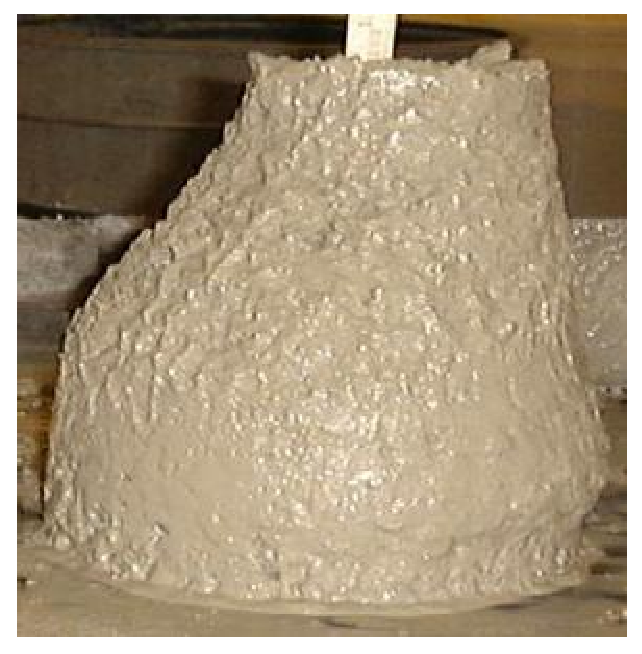
\includegraphics[width=5cm]{slump1b.eps}
  \end{center}
  
\end{frame}

\begin{frame}{}

  {\Large\color{navyblue} Predicting cancer recurrence}

  \begin{center}
    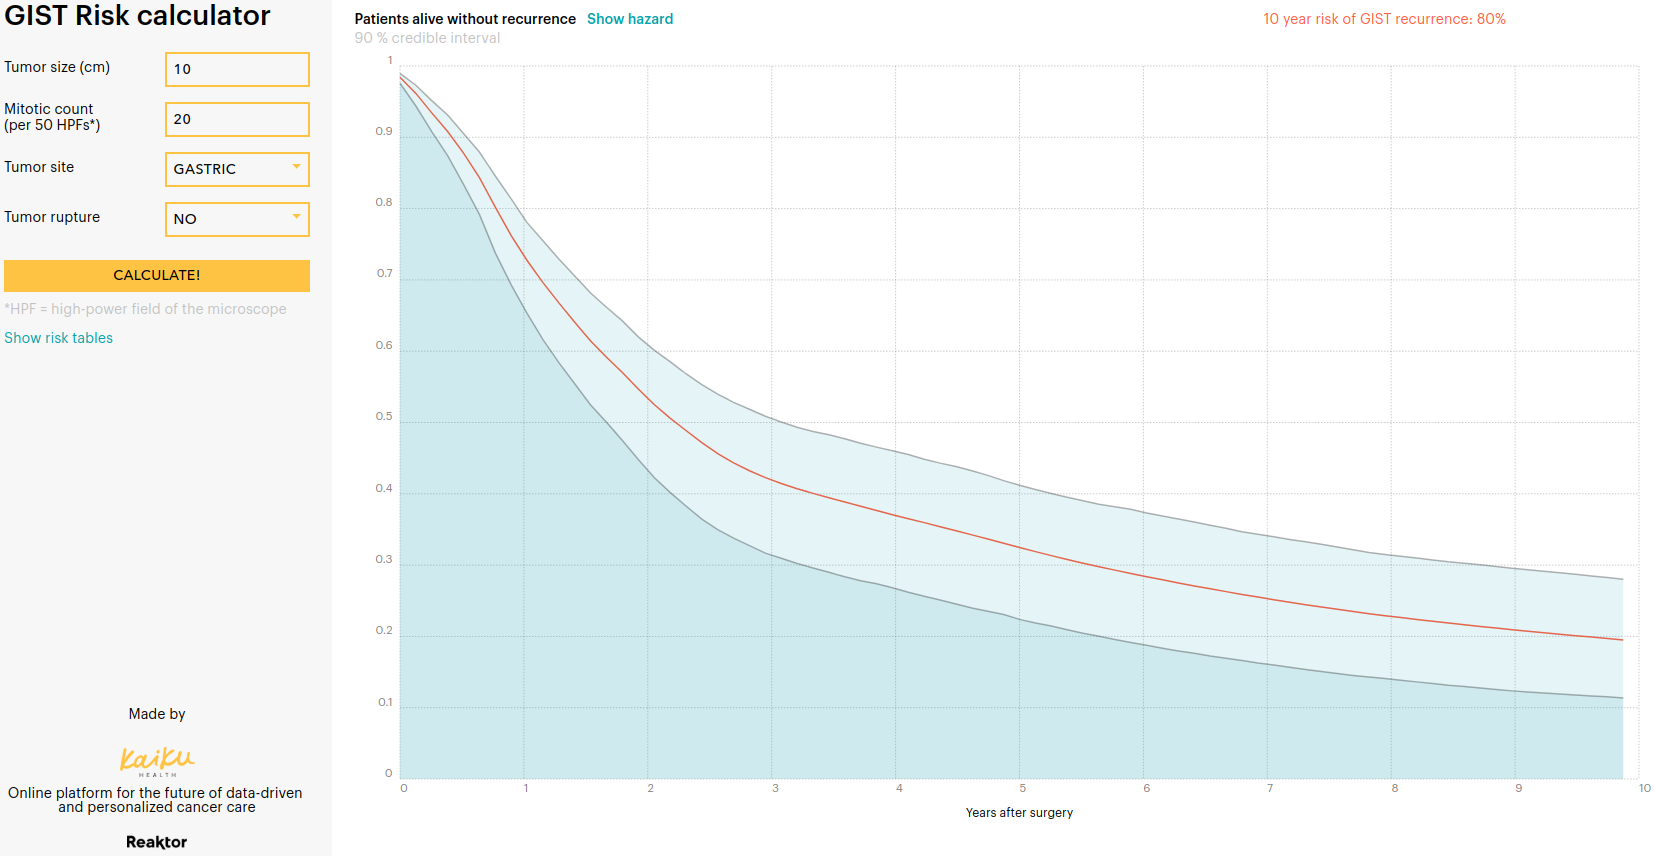
\includegraphics[width=11.5cm]{gistrisk.png}
  \end{center}
  
\end{frame}

\begin{frame}
  
  {\Large\color{navyblue} Predictive performance}

  \begin{itemize}
  \item<1-> True predictive performance is found out by using it to make
    predictions and comparing predictions to true observations
    \begin{itemize}
      \item external validation
    \end{itemize}
  \item<2-> Expected predictive performance
    \begin{itemize}
      \item approximates the external validation
      \end{itemize}
    \end{itemize}

\end{frame}

% \begin{frame}{}

%   {\Large\color{navyblue} Model assessment, comparison, selection and averaging}

%   \begin{list1}
%   \item Modeling complex phenomena with models that
%     are much simpler than the nature ($M$-open)
%   \item<2-> Decision theoretical approch in spirit of
%     \begin{list2}
%     \item Lindley, Box, Rubin, Bernardo \& Smith, etc.
%     \end{list2}
%   \end{list1}
  
% \end{frame}

\begin{frame}
  
  {\Large\color{navyblue} Predictive performance}

  \begin{itemize}
  \item We need to choose the utility/cost function
  \item Application specific utility/cost functions are important
    \begin{itemize}
      \item eg. money, life years, quality adjusted life years, etc.
    \end{itemize}
    \pause
  \item If are interested overall in the goodnes of the predictive distribution,
    or we don't know (yet) the application specific utility, then
    good information theoretically justified choice is log-score
      \begin{align*}
        \log p(y^{\text{rep}} | y, M),
      \end{align*}
\end{itemize}

\end{frame}

\begin{frame}{}
  
  {\Large\color{navyblue} Outline}
  
  \begin{list1}
  \item What is cross-validation
    {\color{gray}
  \begin{list2}
    \item Leave-one-out cross-validation (elpd\_loo, p\_loo)
    \item Uncertainty in LOO (SE)
    \end{list2}
    }
  \item When is cross-validation applicable?
    {\color{gray}
    \begin{list2}
    \item data generating mechanisms and prediction tasks
    \item leave-many-out cross-validation
    \end{list2}
    }
  \item Fast cross-validation
    {\color{gray}
    \begin{list2}
    \item PSIS and diagnostics in loo package (Pareto k, n\_eff, Monte Carlo SE)
    \item K-fold cross-validation
    \end{list2}
    }
  \item {\footnotesize Related methods (WAIC, *IC, BF)}
  \item Model comparison and selection (elpd\_diff, se)
  \item Model averaging with Bayesian stacking
  % \item<2-> Part 2: Projective Inference in High-dimensional Problems:
  %   Prediction and Feature Selection
  \end{list1}
   
\end{frame}

\begin{frame}[fragile]

  {\Large\color{navyblue} Stan and {\tt loo} package}

  {\scriptsize
\begin{lstlisting}
 Computed from 4000 by 20 log-likelihood matrix

         Estimate  SE
elpd_loo    -29.5 3.3
p_loo         2.7 1.0
------
Monte Carlo SE of elpd_loo is 0.1.

Pareto k diagnostic values:
                         Count Pct.    Min. n_eff
(-Inf, 0.5]   (good)     18    90.0%   899       
 (0.5, 0.7]   (ok)        2    10.0%   459       
   (0.7, 1]   (bad)       0     0.0%   <NA>      
   (1, Inf)   (very bad)  0     0.0%   <NA>      

All Pareto k estimates are ok (k < 0.7).
See help('pareto-k-diagnostic') for details.

Model comparison: 
(negative 'elpd_diff' favors 1st model, positive favors 2nd) 

elpd_diff        se 
     -0.2       0.1 
\end{lstlisting}
}

\end{frame}


\begin{frame}{}

  \only<1>{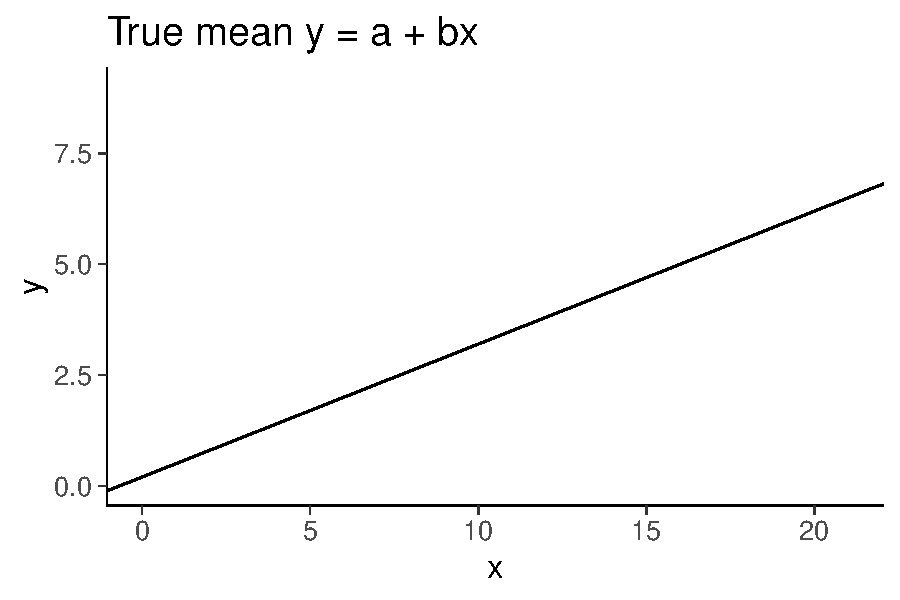
\includegraphics[width=10cm]{fake1.pdf}}
  \only<2>{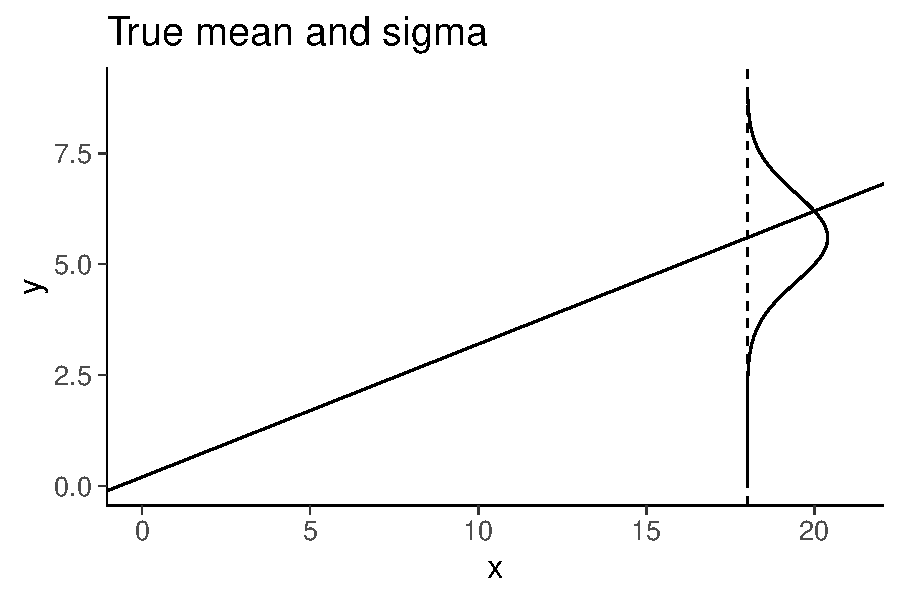
\includegraphics[width=10cm]{fake2.pdf}}
  \only<3>{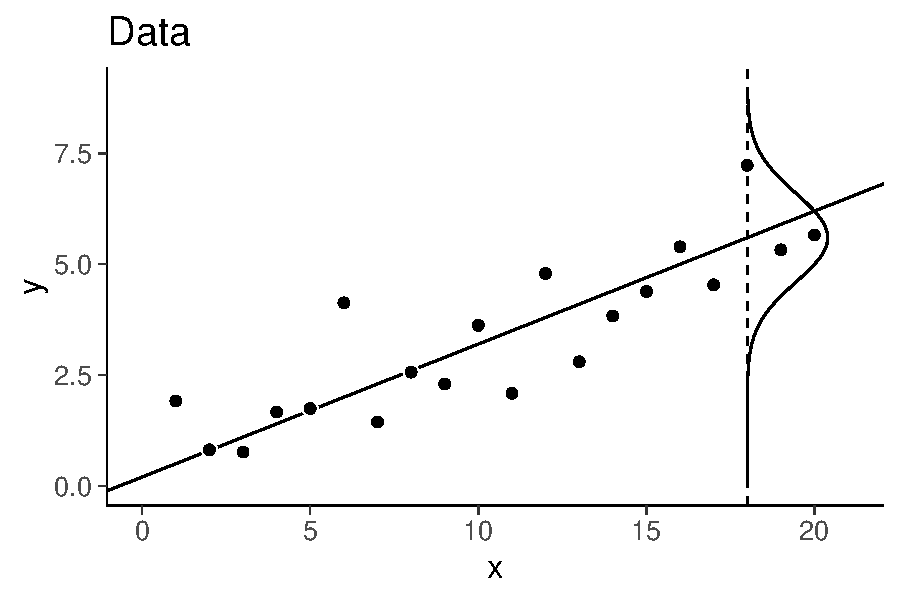
\includegraphics[width=10cm]{fake3.pdf}}
  \only<4>{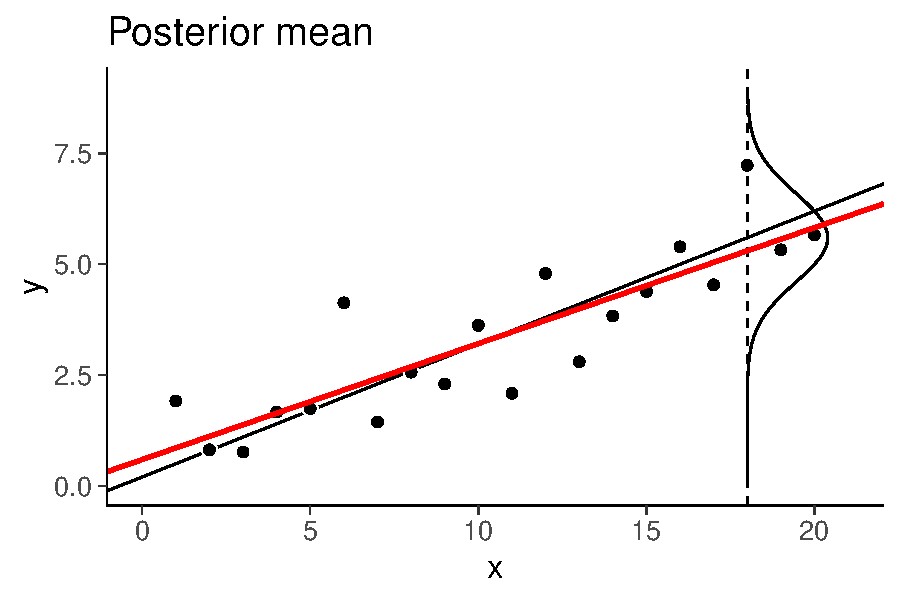
\includegraphics[width=10cm]{fake4.pdf}}
  \only<5>{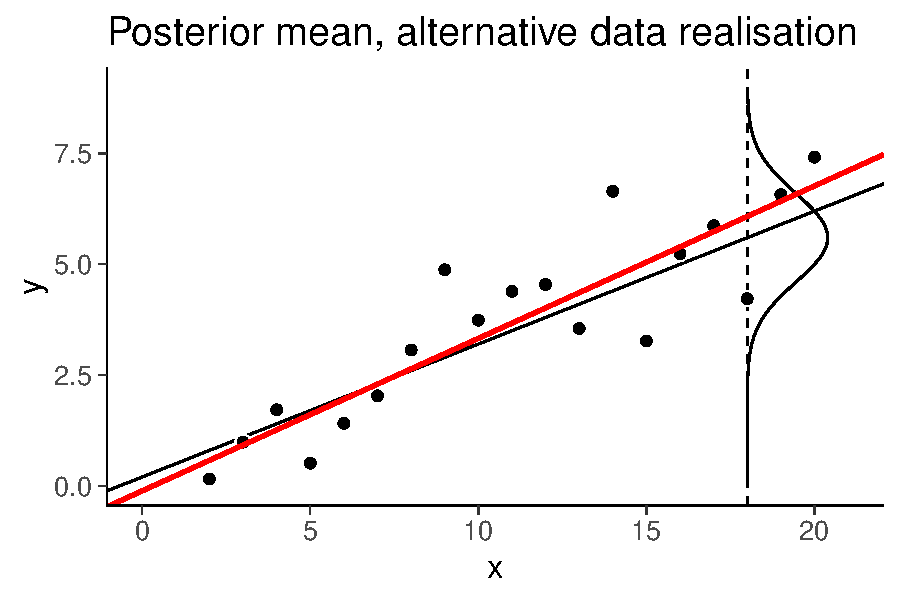
\includegraphics[width=10cm]{fake4b.pdf}}
  \only<6>{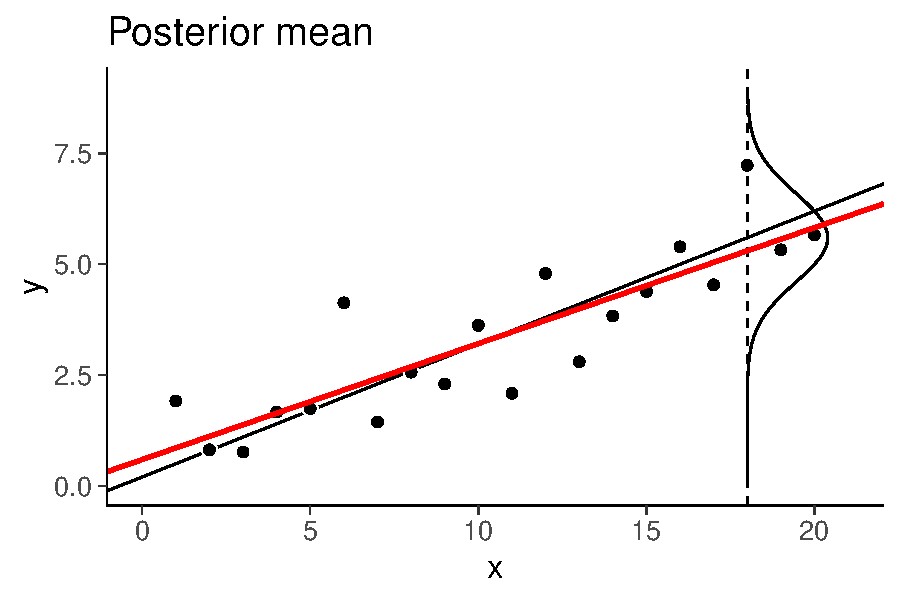
\includegraphics[width=10cm]{fake4.pdf}}
  \only<7>{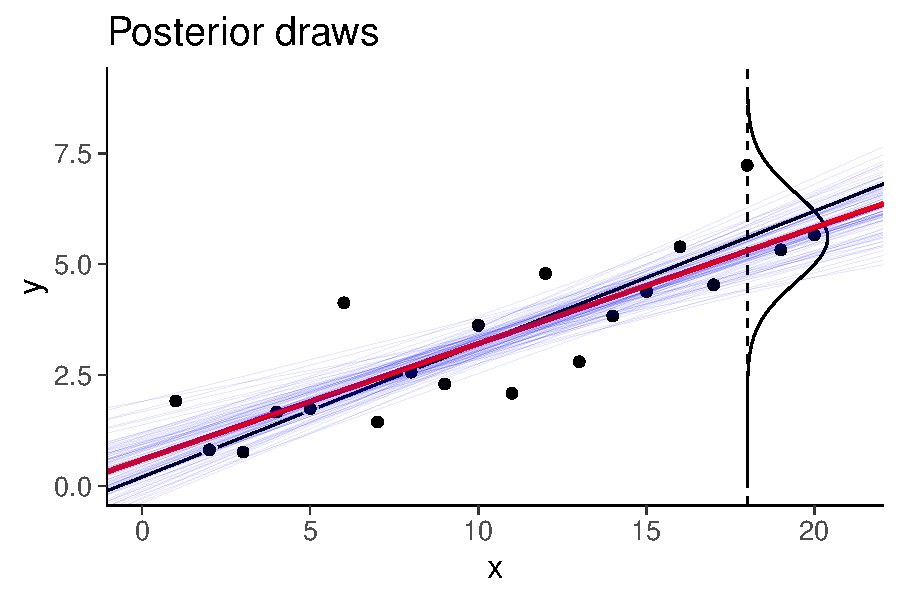
\includegraphics[width=10cm]{fake4s.pdf}}
  \only<8-9>{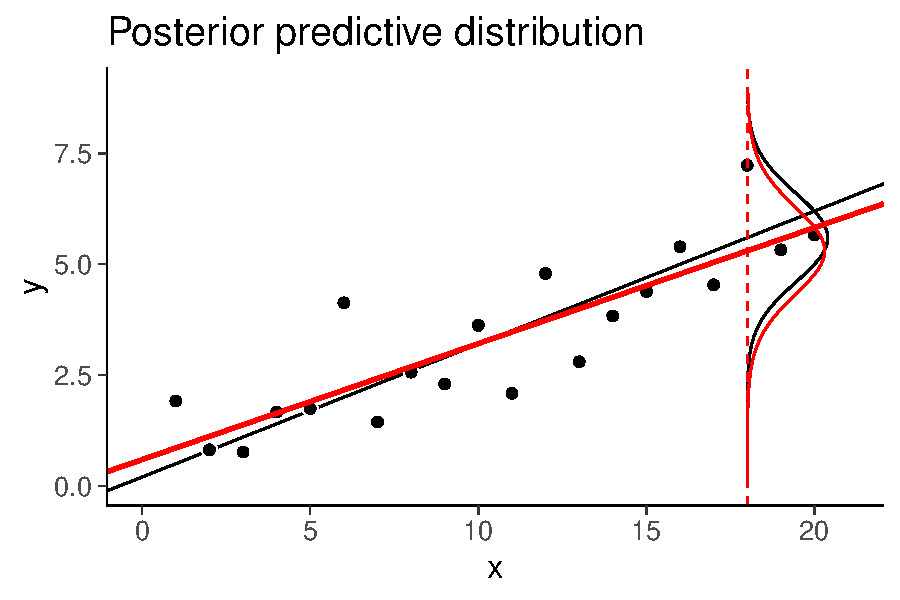
\includegraphics[width=10cm]{fake5.pdf}}
  \only<10>{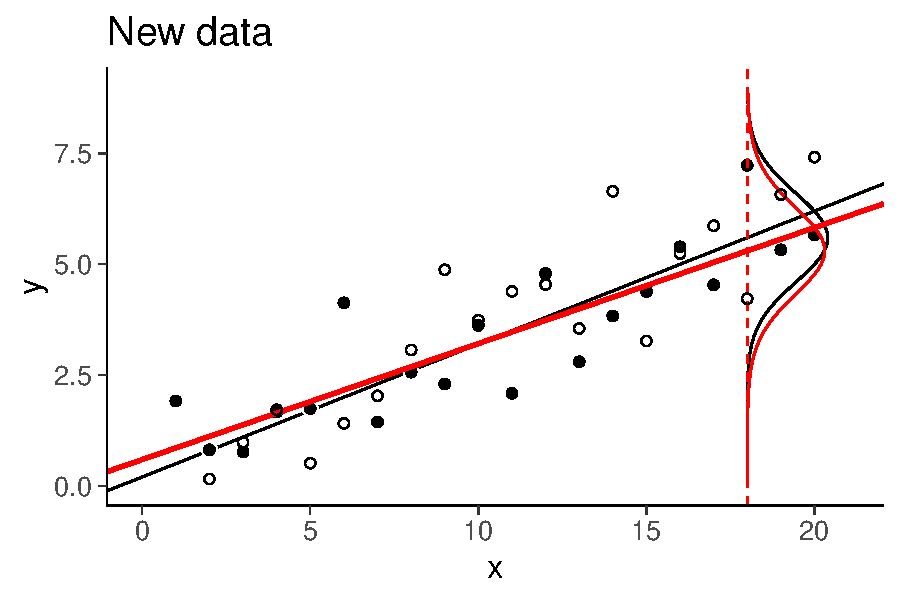
\includegraphics[width=10cm]{fake5n.pdf}}
  \only<11>{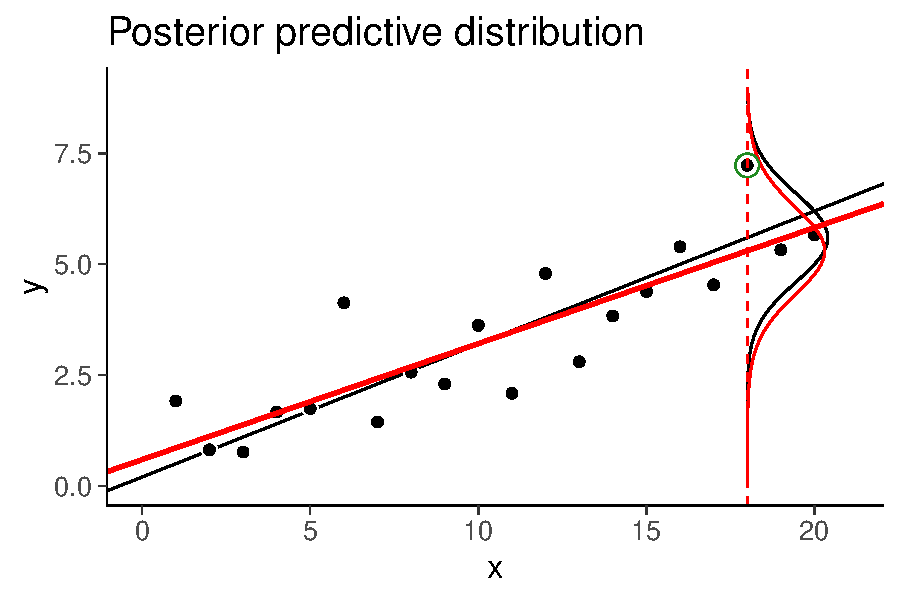
\includegraphics[width=10cm]{fake6.pdf}}
  \only<12>{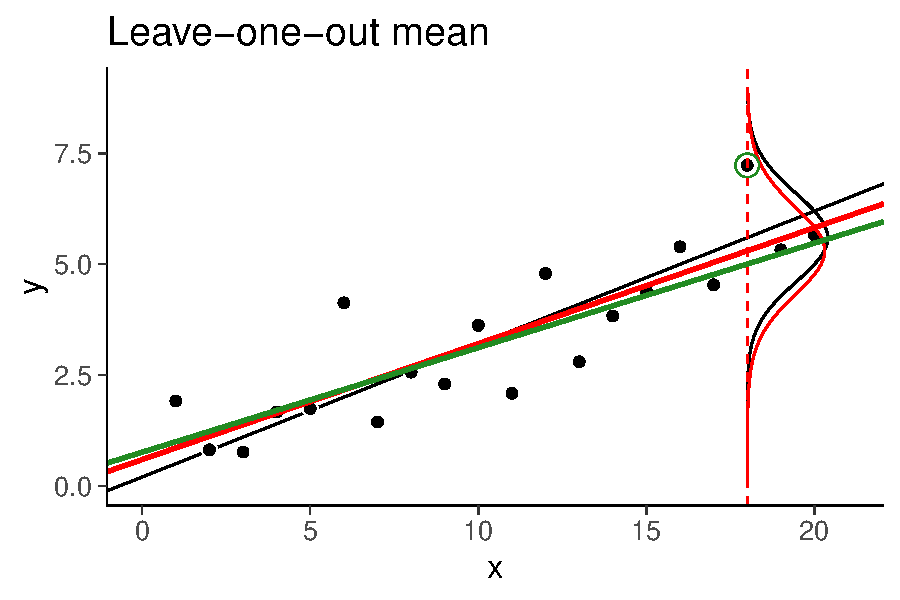
\includegraphics[width=10cm]{fake7.pdf}}
  \\
  \onslide<9>{\color{red} $p(\tilde{y}|\tilde{x}=18,x,y)=\int p(\tilde{y}|\tilde{x}=18,\theta)p(\theta|x,y)d\theta$\\ \vspace{0.5\baselineskip}}
\end{frame}

\begin{frame}{}

  {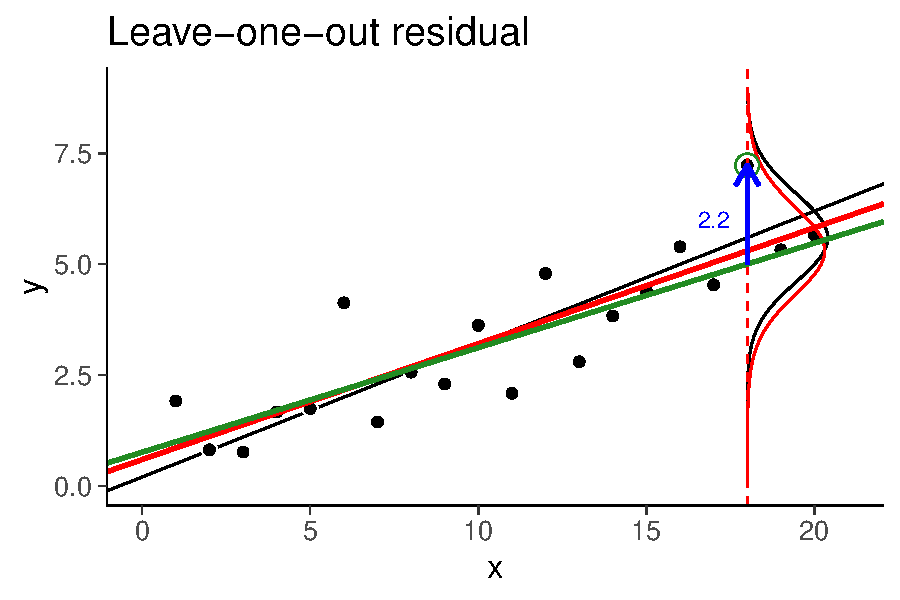
\includegraphics[width=10cm]{fake7r.pdf}}
  \\
  \onslide<2->{{\color{blue} $y_{18} - E[p(\tilde{y}|\tilde{x}=18,x_{-18},y_{-18})]$}\\ \vspace{0.5\baselineskip}}
  \onslide<3->{Can be use to compute, e.g., RMSE, $R^2$, 90\% error}
  \onslide<4>{\\~\\ \small See LOO-$R^2$ at \url{avehtari.github.io/bayes_R2/bayes_R2.html}}
\end{frame}

\begin{frame}{}

  {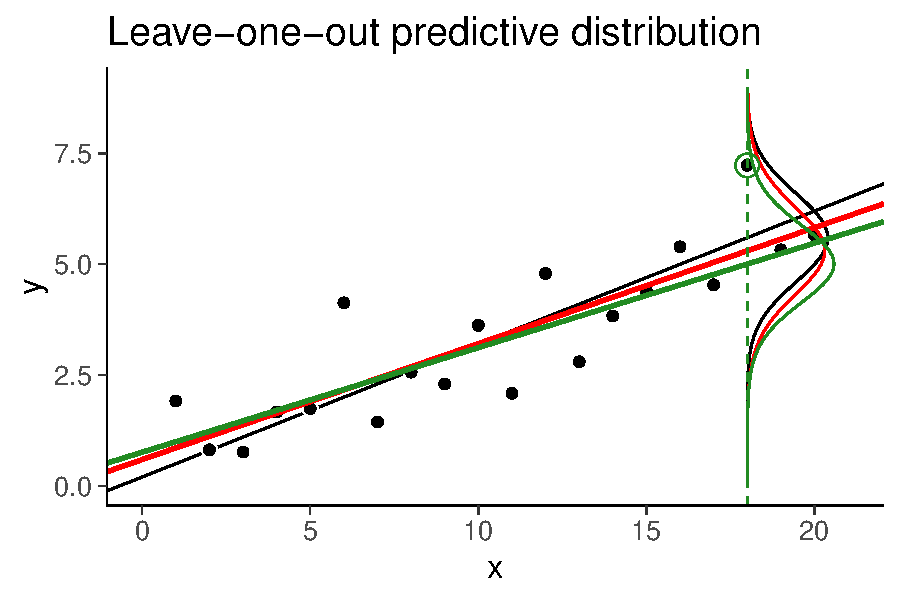
\includegraphics[width=10cm]{fake8.pdf}}
  \\
  \onslide<2>{\color{forestgreen} $p(\tilde{y}|\tilde{x}=18,x_{-18},y_{-18})=\int p(\tilde{y}|\tilde{x}=18,\theta)p(\theta|x_{-18},y_{-18})d\theta$}
  
\end{frame}

\begin{frame}{}

  \only<1-2>{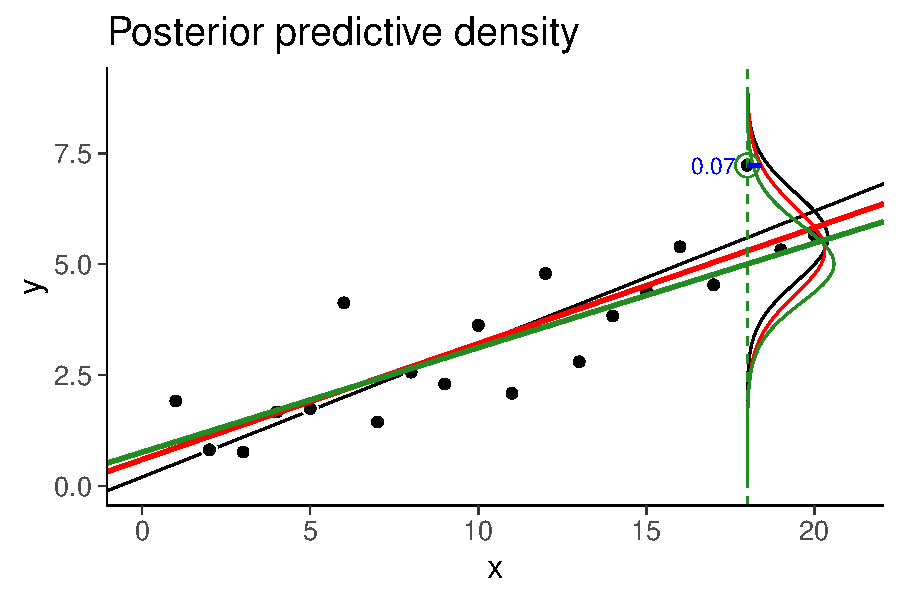
\includegraphics[width=10cm]{fake8pd.pdf}}
  \only<3>{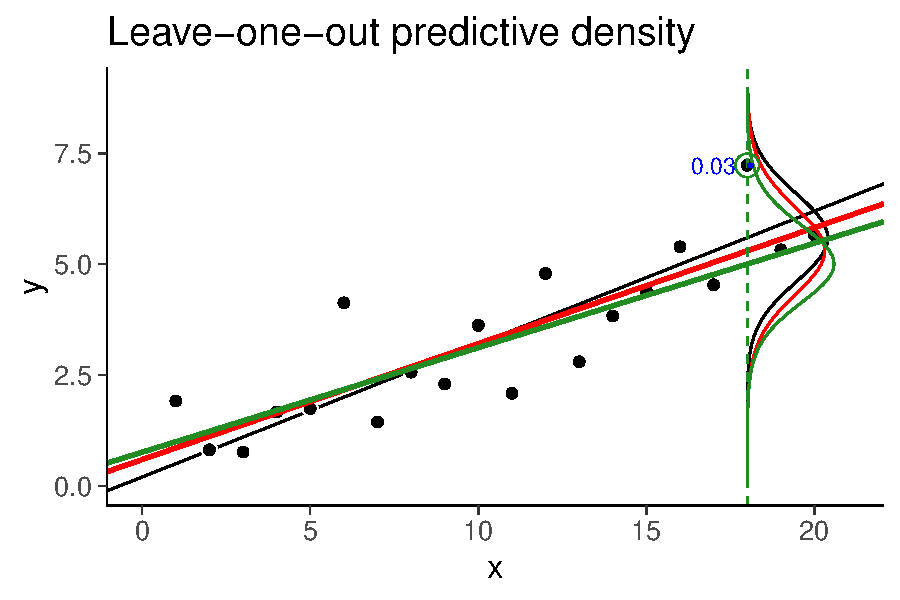
\includegraphics[width=10cm]{fake8loopd.pdf}}
  \\
  \onslide<2->{\color{red} $p(\tilde{y}=y_{18}|\tilde{x}=18,x,y) \approx 0.07$\\ \vspace{0.5\baselineskip}}
  \onslide<3>{\color{forestgreen} $p(\tilde{y}=y_{18}|\tilde{x}=18,x_{-18},y_{-18}) \approx 0.03$}
  
\end{frame}

\begin{frame}{}

  \only<1>{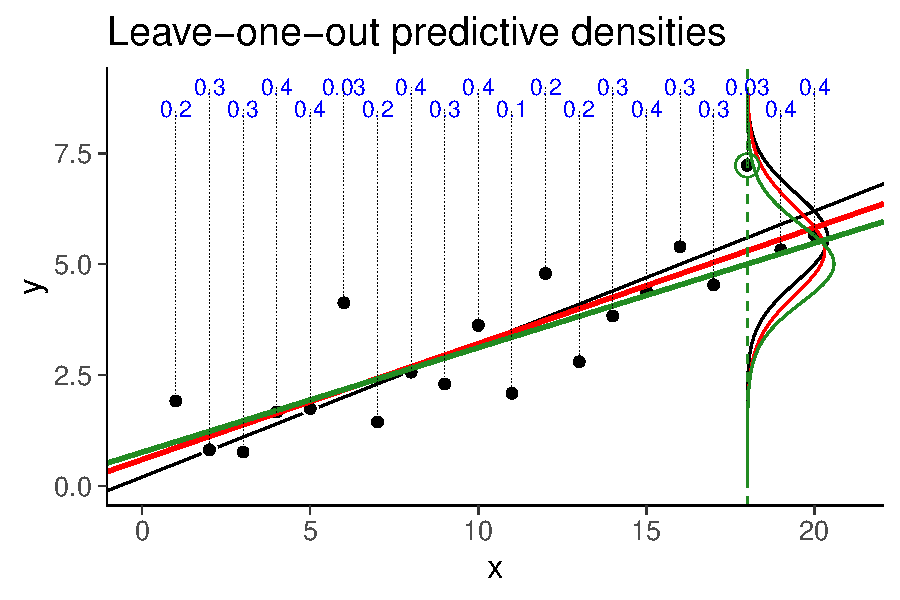
\includegraphics[width=10cm]{fake8loopds.pdf}}
  \only<2->{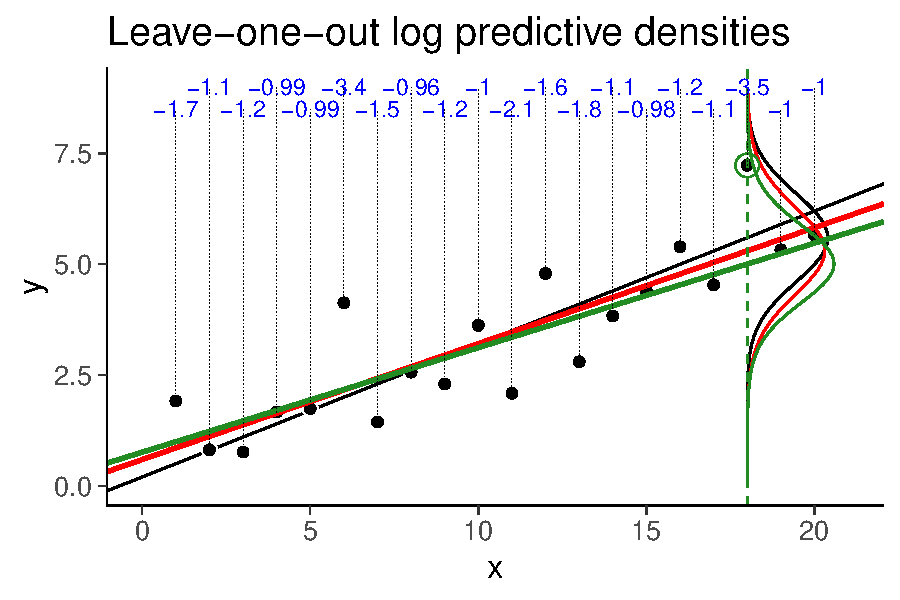
\includegraphics[width=10cm]{fake8loolpds.pdf}}
  \\ \vspace{-0.5\baselineskip}
  \only<1>{\color{blue} $p(y_i|x_i,x_{-i},y_{-i}), \quad i=1,\ldots,20$}
  \only<2>{\color{blue} $\log p(y_i|x_i,x_{-i},y_{-i}), \quad i=1,\ldots,20$}
  \only<3>{\color{blue} $\sum_{i=1}^{20} \log p(y_i|x_i,x_{-i},y_{-i}) \approx -29.5$}
  \only<4->{\color{blue} $\mbox{elpd\_loo} = \sum_{i=1}^{20} \log p(y_i|x_i,x_{-i},y_{-i}) \approx -29.5$\\ \vspace{0.2\baselineskip}}
  \only<5> {\color{blue} unbiased estimate of log posterior pred. density for new data}
  \only<6-7>{\color{red} $\mbox{lpd} = \sum_{i=1}^{20} \log p(y_i|x_i,x,y) \approx -26.8$\\ \vspace{0.2\baselineskip}}
  \only<7>{\color{blue} $\mbox{p\_loo} = \mbox{lpd}-\mbox{elpd\_loo} \approx 2.7$}
  \only<8-> {\color{blue} $\mbox{SE} = \mbox{sd}(\log p(y_i|x_i,x_{-i},y_{-i}))\cdot \sqrt{20} \approx 3.3$}
  \only<9>{\\~\\~\\ \color{black} \footnotesize see \href{http://link.springer.com/article/10.1007/s11222-016-9696-4}{Vehtari, Gelman \& Gabry (2017a)} and \href{http://dx.doi.org/10.1214/12-SS102}{Vehtari \& Ojanen (2012)} for more}
  
\end{frame}

\begin{frame}{}

  \only<1>{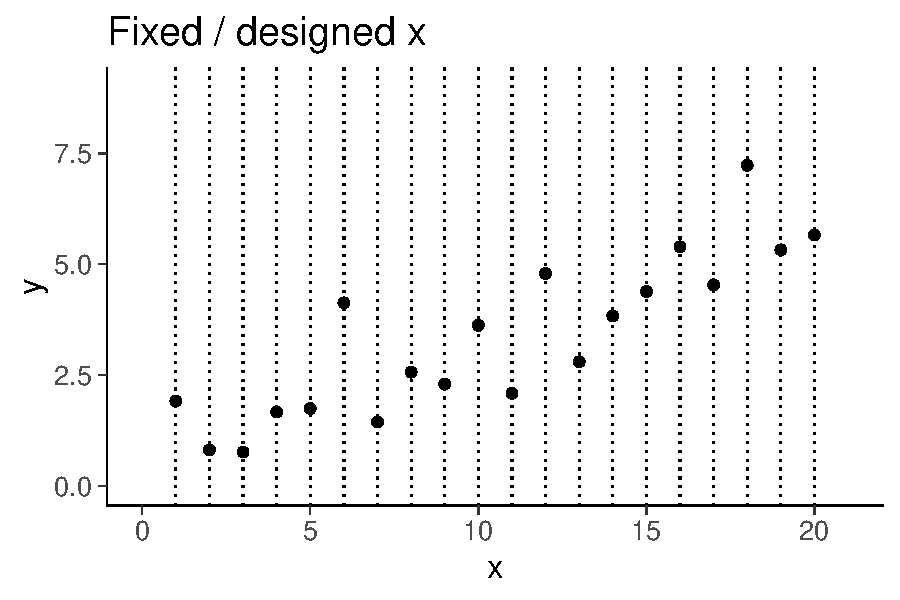
\includegraphics[width=10cm]{fakedfixed.pdf}}
  \only<2->{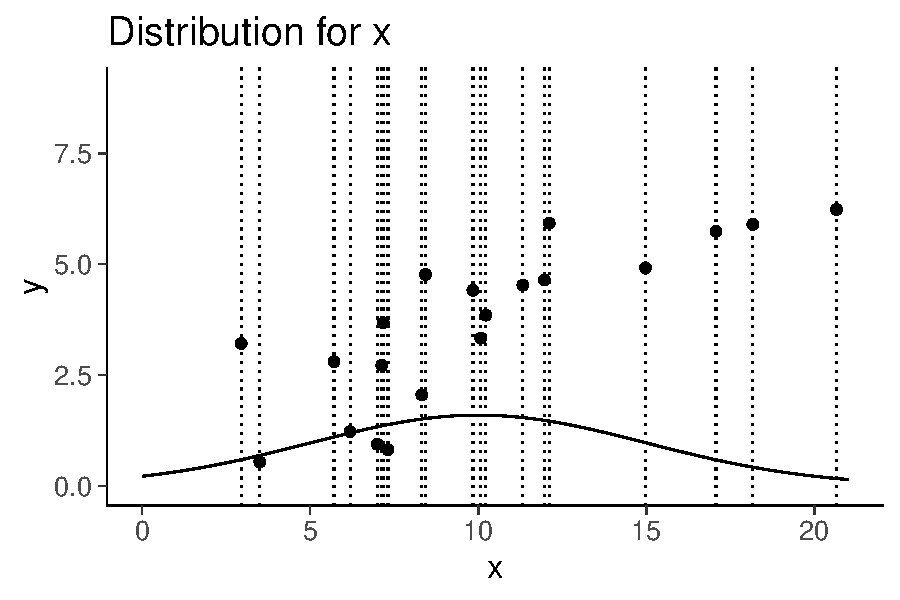
\includegraphics[width=10cm]{fakedrandom.pdf}}
  \\ \vspace{-0.5\baselineskip}
  \only<1>{LOO is ok for fixed / designed $x$. SE is uncertainty about $y|x$.\\ \vspace{0.2\baselineskip}}
  \only<2->{LOO is ok for random $x$. SE is uncertainty about $y|x$ and $x$.\\ \vspace{0.2\baselineskip}}
  \onslide<3>{Covariate shift can be handled with importance weighting or modelling}
  \onslide<1->{\\ \small see \href{http://dx.doi.org/10.1214/12-SS102}{Vehtari \& Ojanen (2012)} and \url{andrewgelman.com/2018/08/03/loo-cross-validation-approaches-valid/}}
  
\end{frame}

\begin{frame}[fragile]

  {\Large\color{navyblue} {\tt loo} package}

  {\scriptsize
\begin{lstlisting}
 Computed from 4000 by 20 log-likelihood matrix

         Estimate  SE
elpd_loo    -29.5 3.3
p_loo         2.7 1.0
\end{lstlisting}
      {\color{gray}
\begin{lstlisting}
------
Monte Carlo SE of elpd_loo is 0.1.

Pareto k diagnostic values:
                         Count Pct.    Min. n_eff
(-Inf, 0.5]   (good)     18    90.0%   899       
 (0.5, 0.7]   (ok)        2    10.0%   459       
   (0.7, 1]   (bad)       0     0.0%   <NA>      
   (1, Inf)   (very bad)  0     0.0%   <NA>      

All Pareto k estimates are ok (k < 0.7).
See help('pareto-k-diagnostic') for details.
\end{lstlisting}}
}
\end{frame}

\begin{frame}{}

  \only<1>{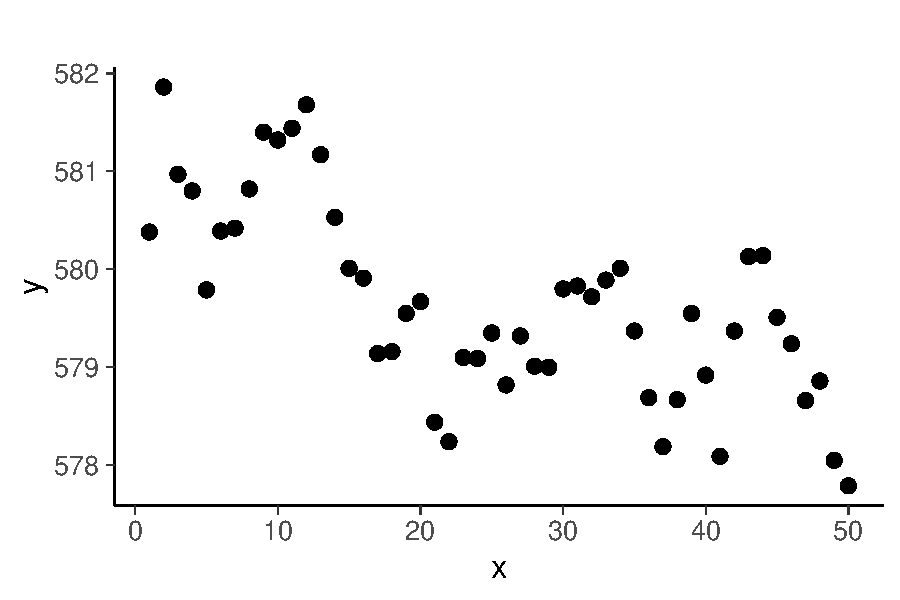
\includegraphics[width=10cm]{lake1data.pdf}}
  \only<2>{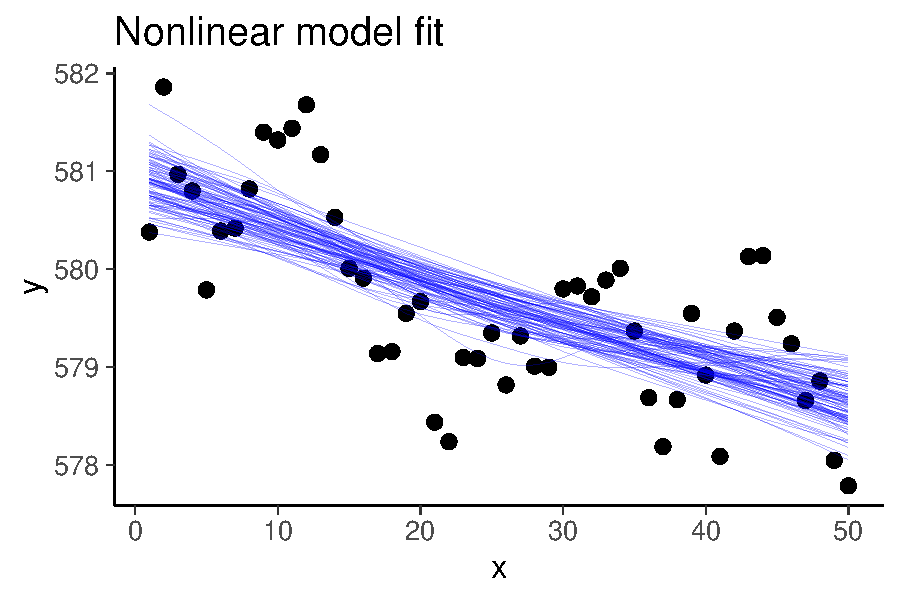
\includegraphics[width=10cm]{lake1gp.pdf}}
  \only<3->{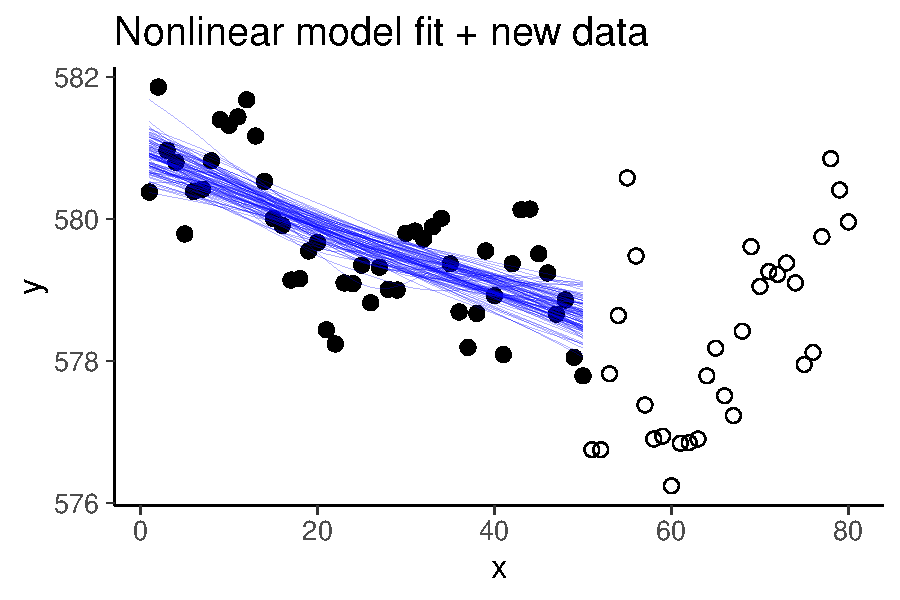
\includegraphics[width=10cm]{lake1gpptest.pdf}}
  \\
  \only<4>{Extrapolation is more difficult}
  
\end{frame}

\begin{frame}{}

  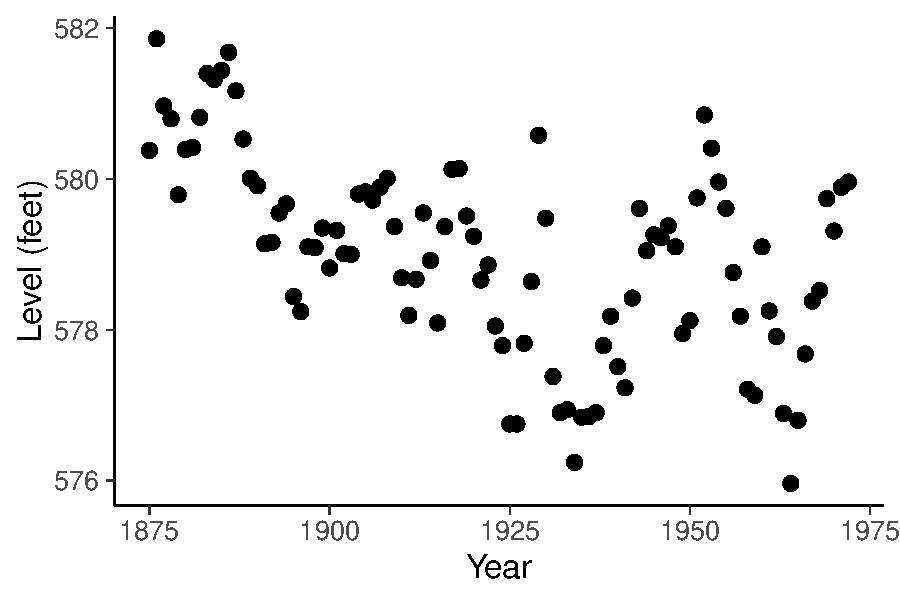
\includegraphics[width=10cm]{lake2data.pdf}

  
  {Can LOO or other cross-validation be used with time series?}
  
\end{frame}

\begin{frame}{}

  \only<1>{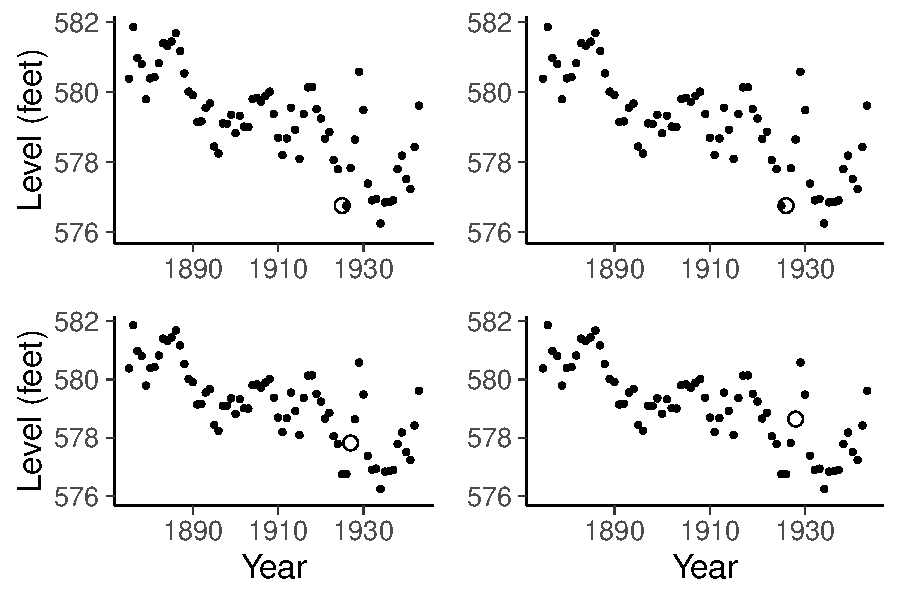
\includegraphics[width=10cm]{lake3loo.pdf}}
  \only<2>{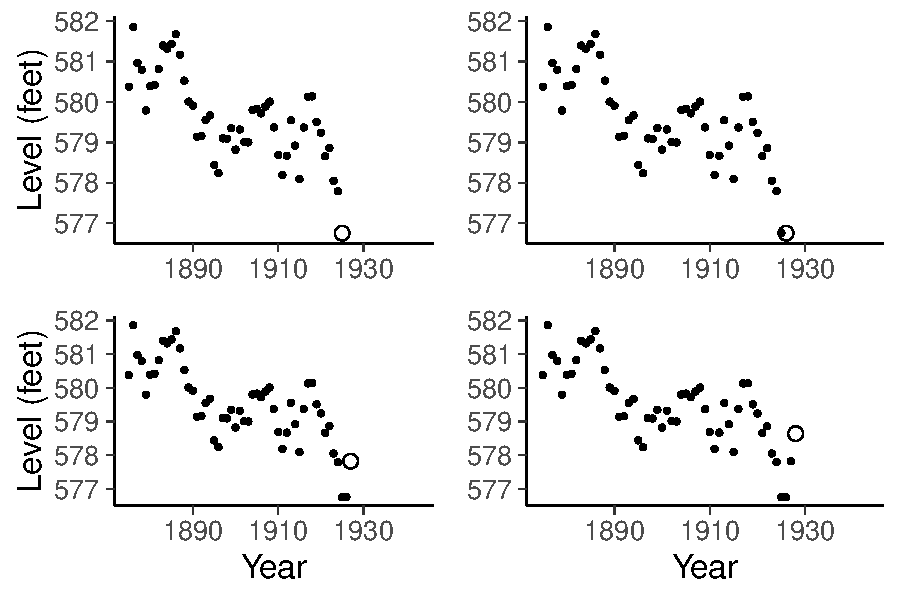
\includegraphics[width=10cm]{lake3stepahead.pdf}}
  \only<3>{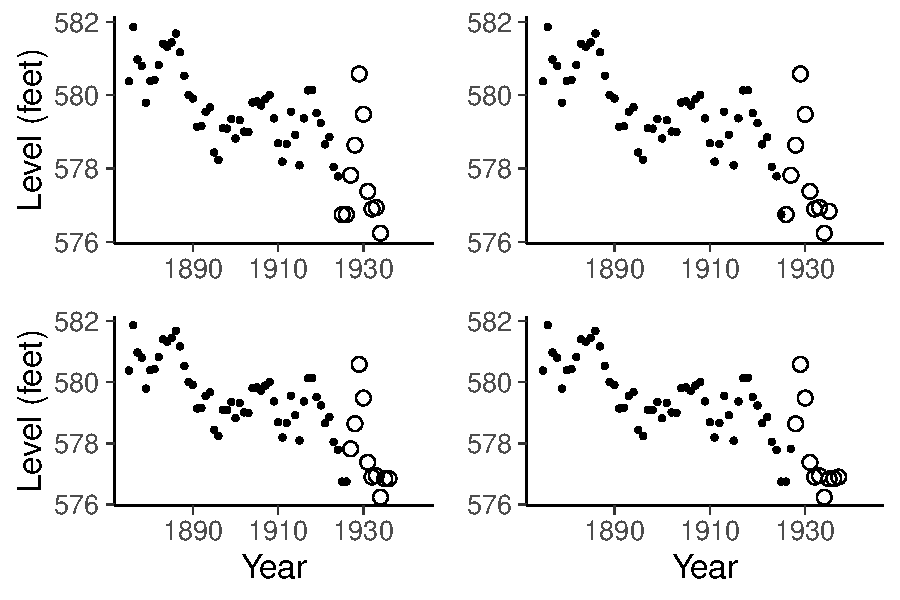
\includegraphics[width=10cm]{lake3tenstepahead.pdf}}
  \only<4>{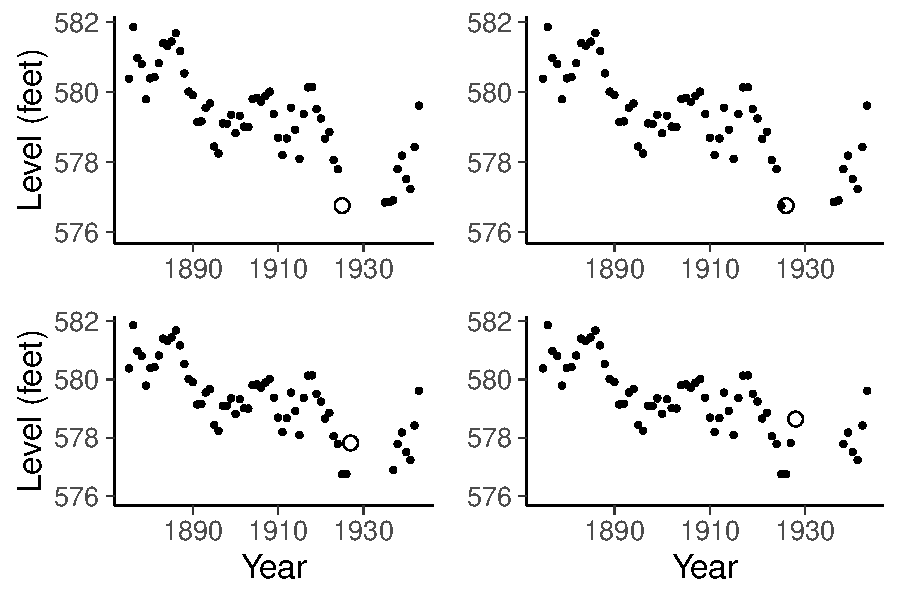
\includegraphics[width=10cm]{lake3stepaheadblock.pdf}}
  \\
  \only<1>{Leave-one-out cross-validation is ok for assessing conditional model}
  \only<2>{Leave-future-out cross-validation is better for predicting future}
  \only<3>{$m$-step-ahead cross-validation is better for predicting further future}
  \only<4>{$m$-step-ahead leave-a-block-out cross-validation}
  
\end{frame}

\begin{frame}{}

  \only<1>{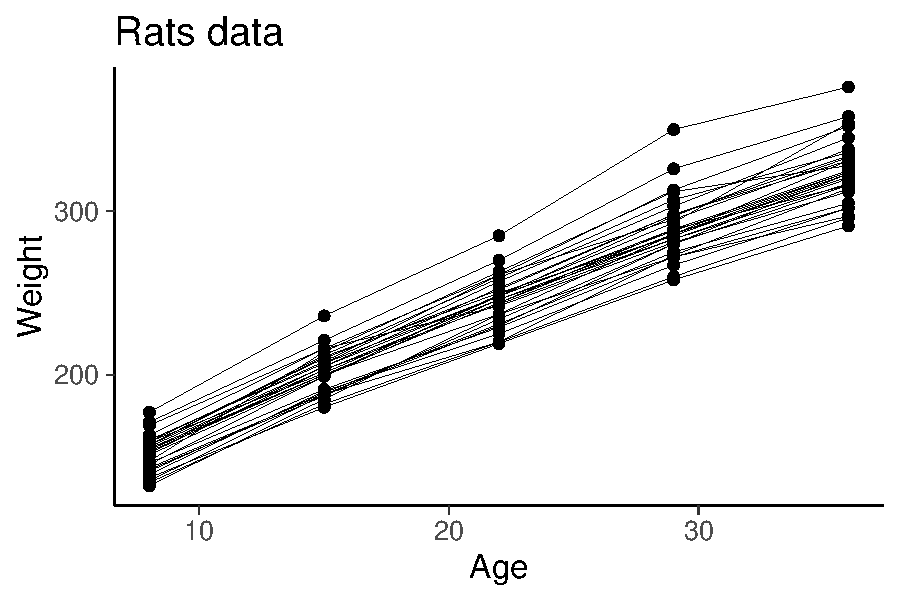
\includegraphics[width=10cm]{rats1data.pdf}}
  \only<2>{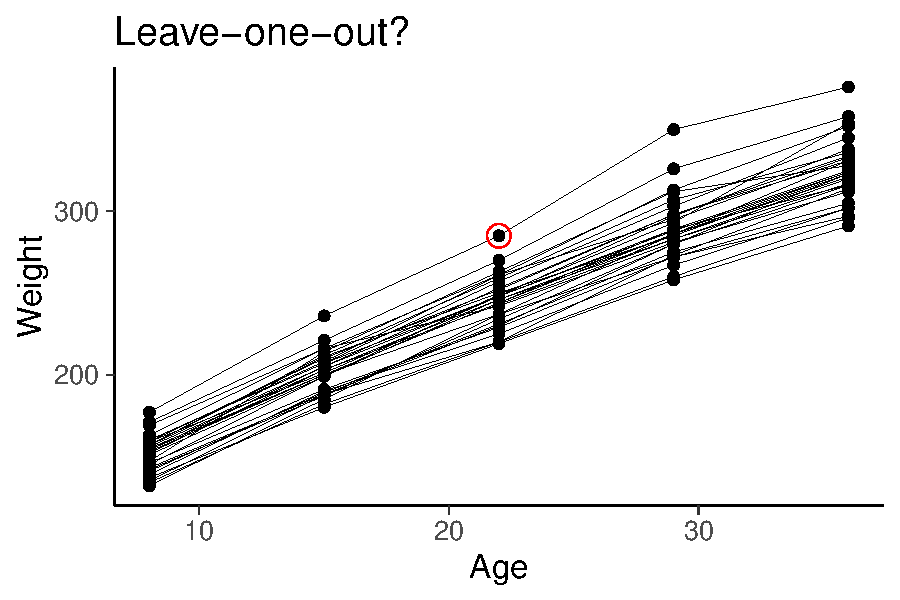
\includegraphics[width=10cm]{rats1loo.pdf}}
  \only<3>{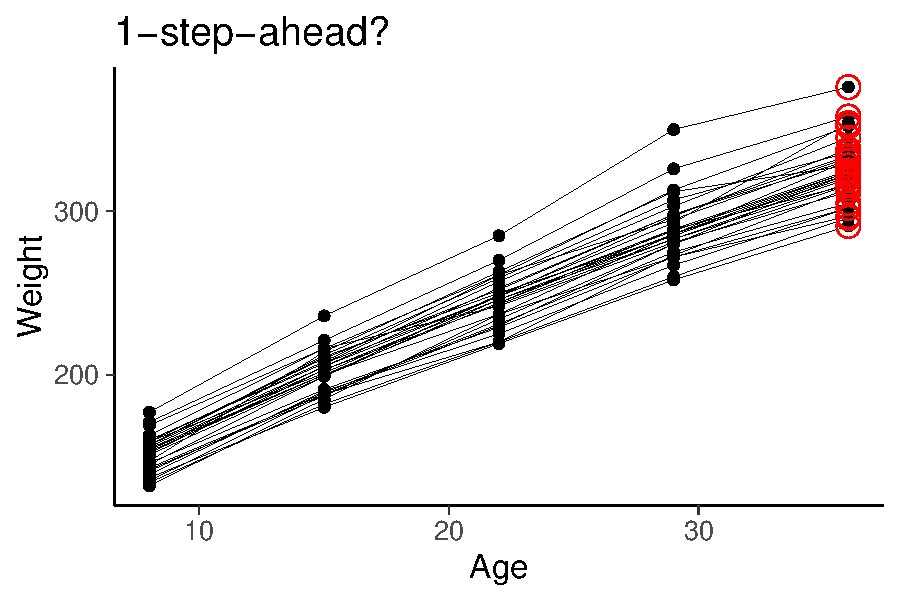
\includegraphics[width=10cm]{rats1step.pdf}}
  \only<4>{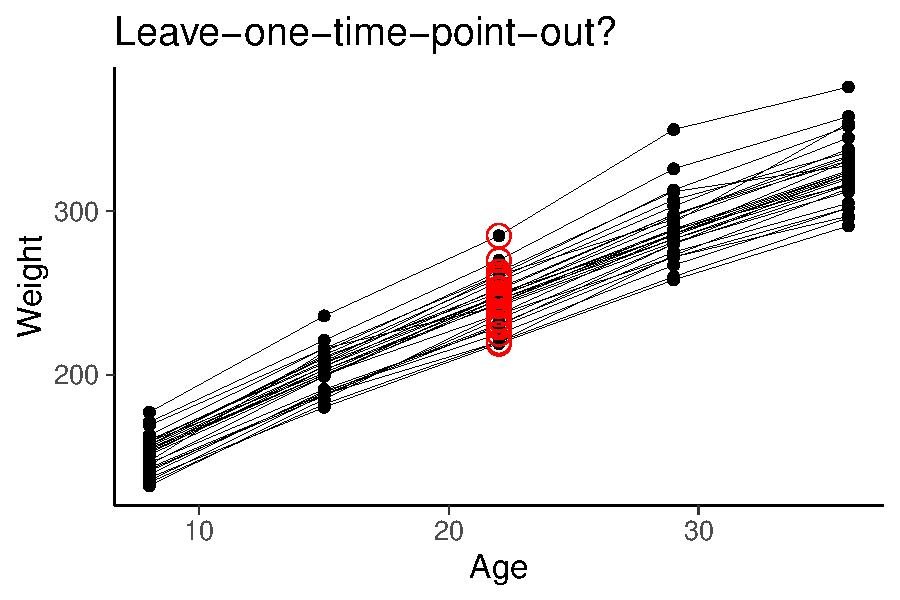
\includegraphics[width=10cm]{rats1onetime.pdf}}
  \only<5>{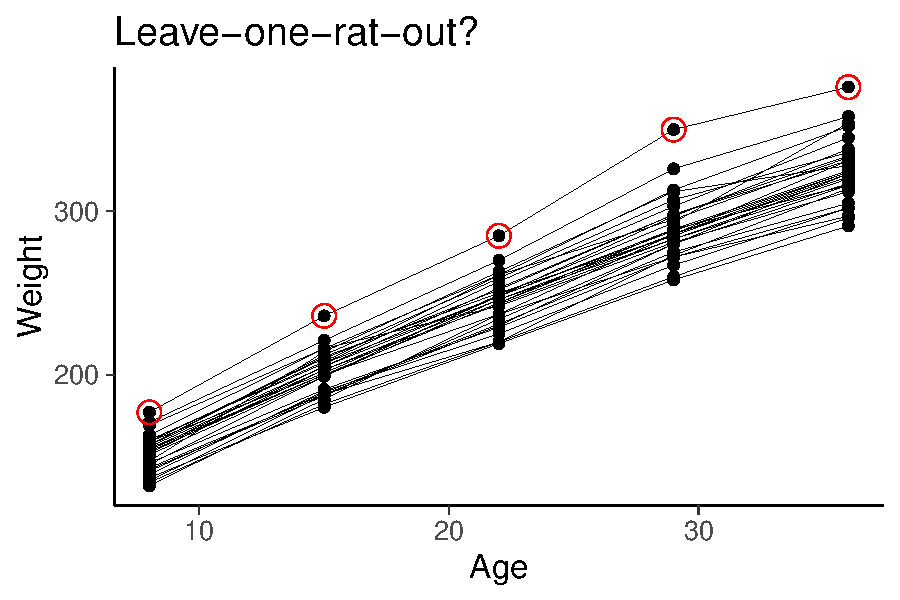
\includegraphics[width=10cm]{rats1onerat.pdf}}
  \only<6>{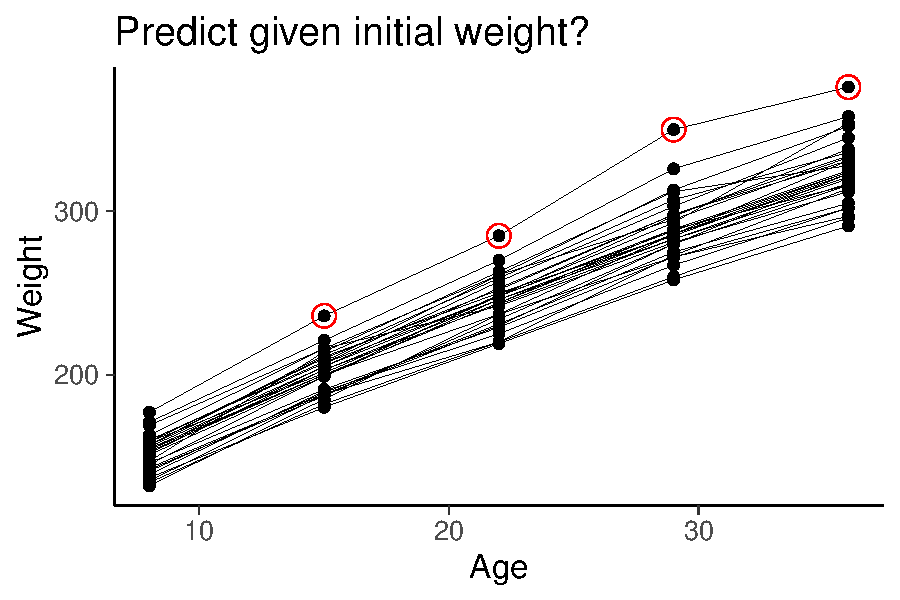
\includegraphics[width=10cm]{rats1init.pdf}}
  \\
  \only<1>{Can LOO or other cross-validation be used with hierarchical data?}
  \only<2->{Yes!}
  
\end{frame}

\begin{frame}{}

{\Large\color{navyblue} Summary of data generating mechanisms and prediction tasks}

\begin{list1}
\item You have to make some assumptions on data generating mechanism
\item Use the knowledge of the prediction task if available
\item Cross-validation can be used to analyse different parts, even if
  there is no clear prediction task
\end{list1}

 \vspace{6.5\baselineskip}
{ \small see \href{http://dx.doi.org/10.1214/12-SS102}{Vehtari \& Ojanen (2012)} and \url{andrewgelman.com/2018/08/03/loo-cross-validation-approaches-valid/}}

\end{frame}

\begin{frame}{}

{\Large\color{navyblue} Fast cross-validation}

\begin{list1}
\item Pareto smoothed importance sampling LOO (PSIS-LOO)
\item K-fold cross-validation
\end{list1}

\vspace{12\baselineskip}

{\small see \href{http://link.springer.com/article/10.1007/s11222-016-9696-4}{Vehtari, Gelman \& Gabry (2017a)} and \url{mc-stan.org/loo/}}

\end{frame}

\begin{frame}{}

  \only<1>{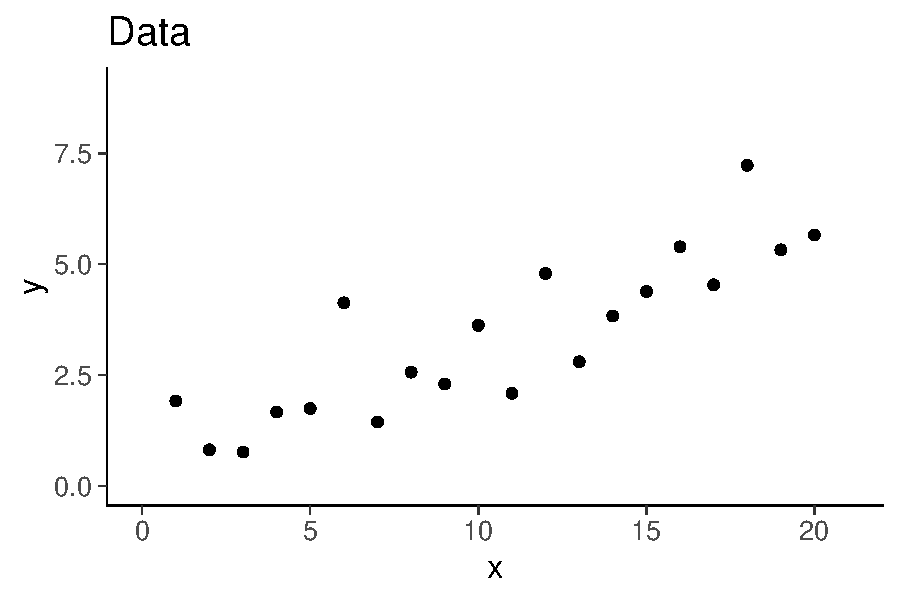
\includegraphics[width=10cm]{fakedata.pdf}}
  \only<2>{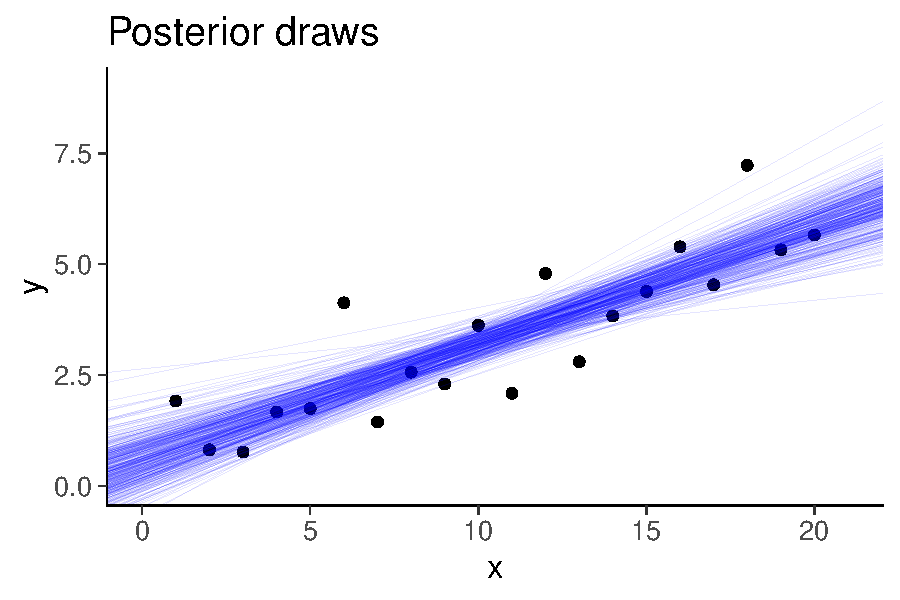
\includegraphics[width=10cm]{fakedraws.pdf}}
  \only<3>{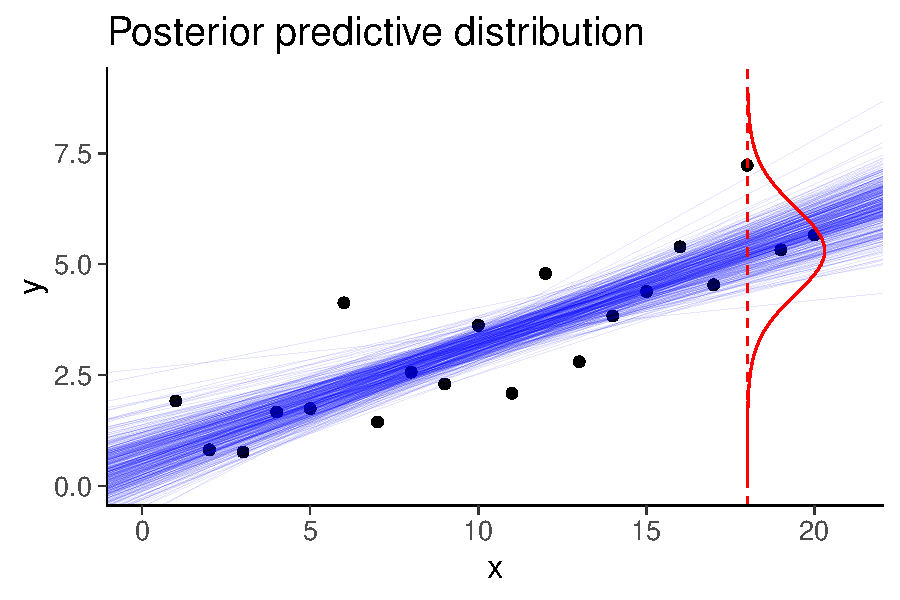
\includegraphics[width=10cm]{fakepostpred.pdf}}
  \only<4>{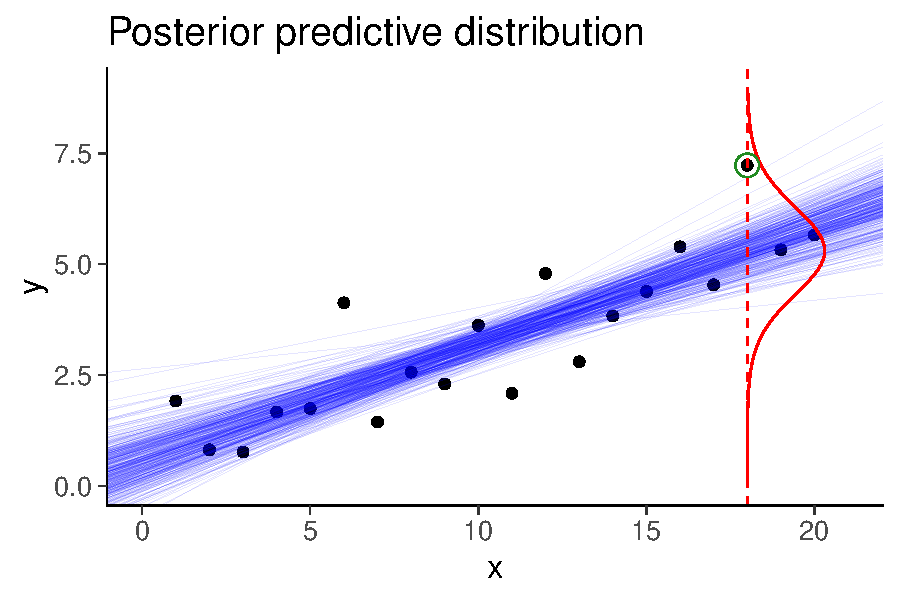
\includegraphics[width=10cm]{fakepostpred18.pdf}}
  \only<5-7>{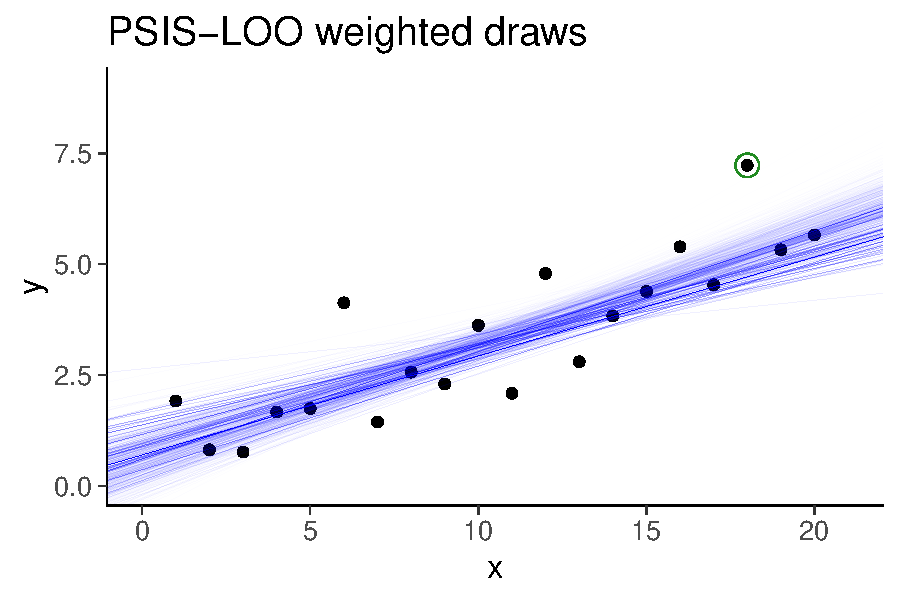
\includegraphics[width=10cm]{fakepsisdraws.pdf}}
  \only<8-10>{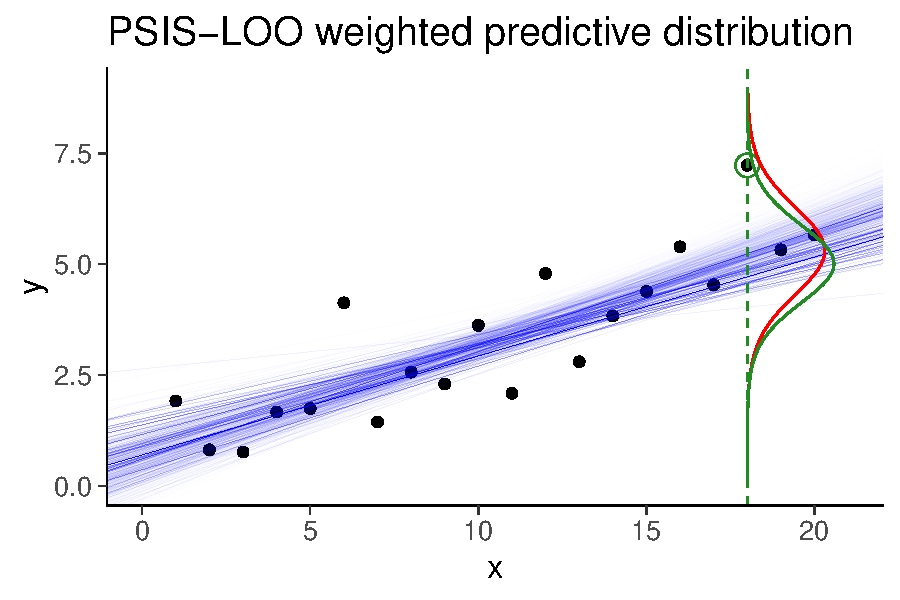
\includegraphics[width=10cm]{fakepsispostpred.pdf}}
  \\
  \only<2>{$\theta^{(s)} \sim p(\theta|x,y)$}
  \only<3-4>{$\theta^{(s)} \sim p(\theta|x,y), \quad p(\tilde{y}|\tilde{x},x,y) \approx \frac{1}{S}\sum_{s=1}^S p(\tilde{y}|\tilde{x},\theta^{(s)})$ }
  \only<5>{$\theta^{(s)} \sim p(\theta|x,y)$\\ \vspace{0.2\baselineskip}$ r_i^{(s)} = p(\theta^{(s)}|x_{-i},y_{-i}) / p(\theta^{(s)}|x,y)$ }
  \only<6-8>{$\theta^{(s)} \sim p(\theta|x,y)$\\ \vspace{0.2\baselineskip} $ r_i^{(s)} = p(\theta^{(s)}|x_{-i},y_{-i}) / p(\theta^{(s)}|x,y) \propto 1/p(y_i|x_i,\theta^{(s)})$\\ \vspace{0.2\baselineskip} }
  \only<7>{$\log(1/p(y_i|x_i,\theta^{(s)})) = -\mbox{log\_lik}[i]$}
  \only<9-10>{$\theta^{(s)} \sim p(\theta|x,y)$\\ \vspace{0.2\baselineskip}
    $ r_i^{(s)} = p(\theta^{(s)}|x_{-i},y_{-i}) / p(\theta^{(s)}|x,y) \propto 1/p(y_i|x_i,\theta^{(s)})$\\ \vspace{0.2\baselineskip}
  $p(y_i|x_i,x_{-i},y_{-i}) \approx \sum_{s=1}^S [w_i^{(s)} p(y_i|x_i,\theta^{(s)})]$}\only<10>{, where $w \leftarrow \mbox{PSIS}(r)$}
  
\end{frame}

\begin{frame}{}

  \only<1>{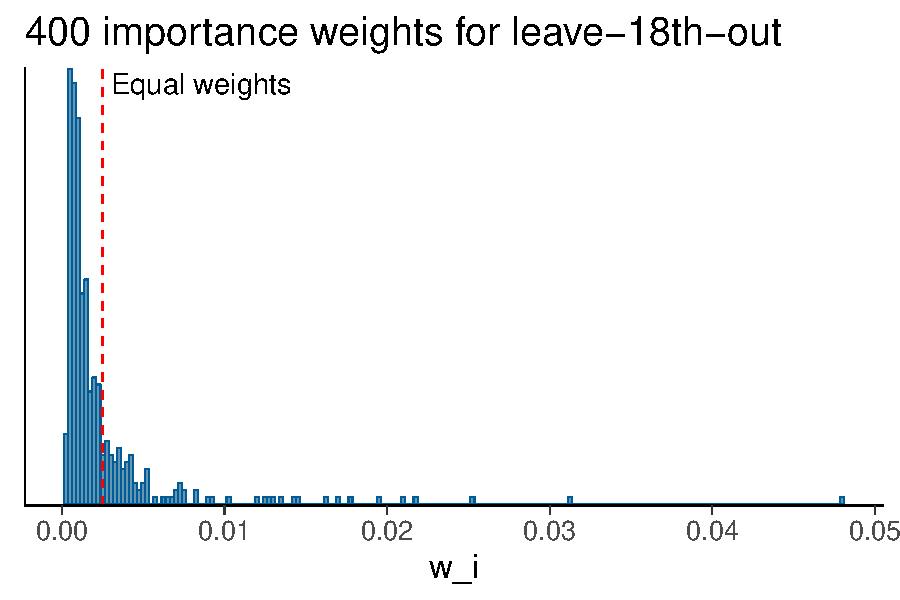
\includegraphics[width=10cm]{fakepsisweights.pdf}}
  \only<2->{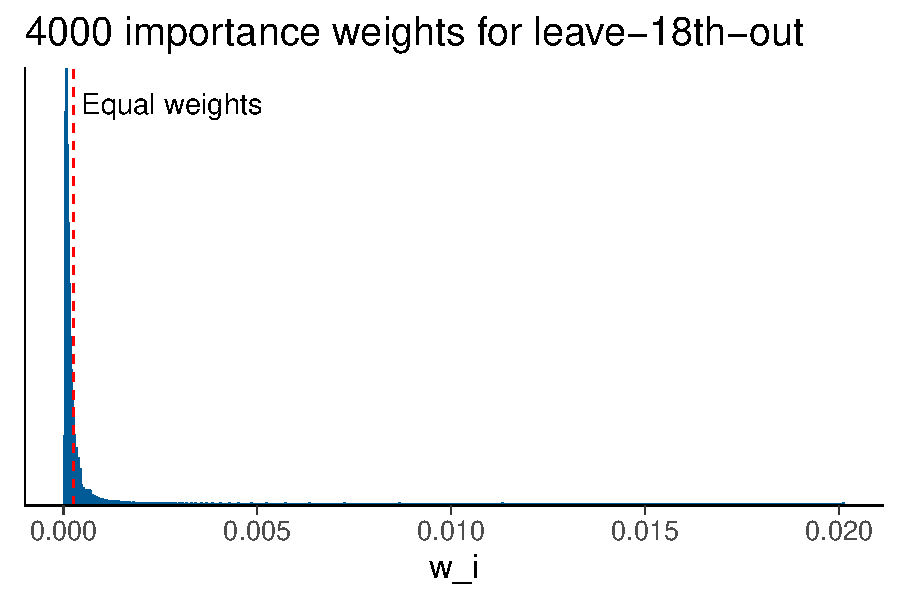
\includegraphics[width=10cm]{fakepsisweights4000.pdf}}
  \\
  \vspace{-\baselineskip}
  \onslide<3->{n\_eff $\approx$ 459\\  \vspace{0.2\baselineskip}}
  \onslide<4>{Pareto $\hat{k}$ $\approx$ 0.52
  \vspace{-\parskip}
    \begin{list2}
    \item Pareto $\hat{k}$ estimates the tail shape which determines the convergence rate of PSIS. Less than 0.7 is ok.}
\end{list2}
  \onslide<3->{\vspace{0.1\baselineskip}\small see \href{http://link.springer.com/article/10.1007/s11222-016-9696-4}{Vehtari, Gelman \& Gabry (2017b)}}
\end{frame}

\begin{frame}[fragile]

  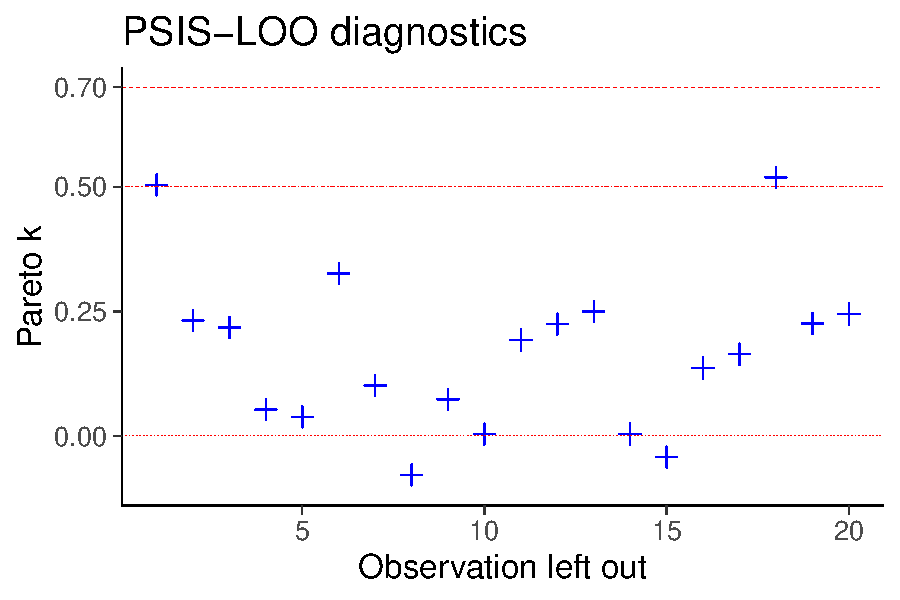
\includegraphics[width=10cm]{fakepks.pdf}

\end{frame}

\begin{frame}[fragile]

  \only<1>{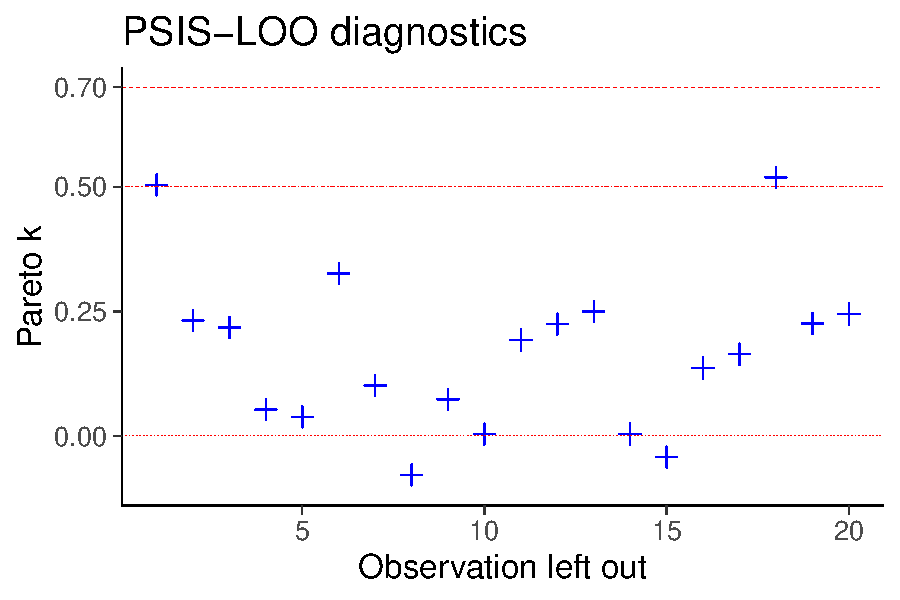
\includegraphics[width=10cm]{fakepks.pdf}}
  \only<2>{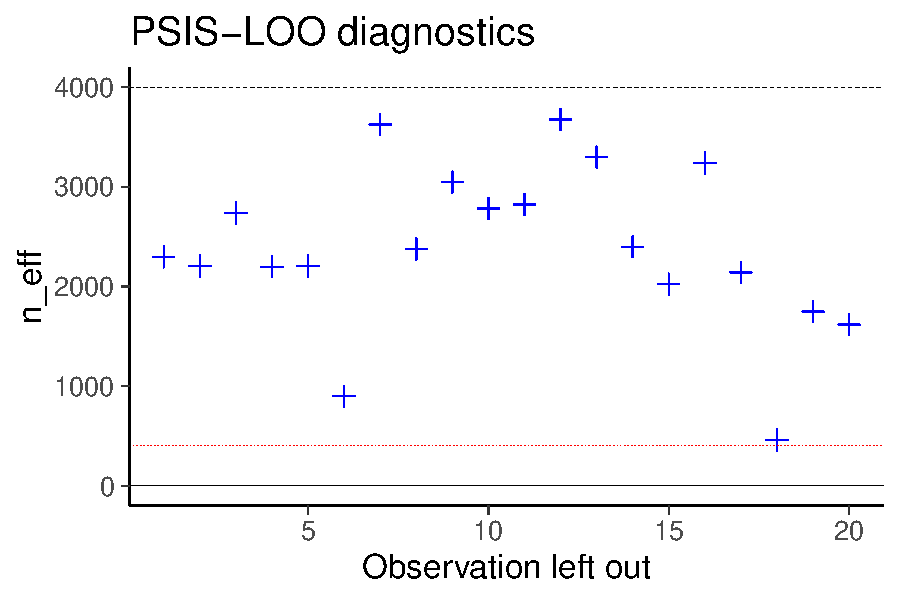
\includegraphics[width=10cm]{fakeneffs.pdf}}
  \\
  {\scriptsize
\begin{lstlisting}
    Pareto k diagnostic values:
                         Count Pct.    Min. n_eff
(-Inf, 0.5]   (good)     18    90.0%   899       
 (0.5, 0.7]   (ok)        2    10.0%   459       
   (0.7, 1]   (bad)       0     0.0%   <NA>      
   (1, Inf)   (very bad)  0     0.0%   <NA>      
\end{lstlisting}
}

\end{frame}

\begin{frame}[fragile]

  {\Large\color{navyblue} {\tt loo} package}

  {\scriptsize
    {\color{gray}
\begin{lstlisting}
 Computed from 4000 by 20 log-likelihood matrix

         Estimate  SE
elpd_loo    -29.5 3.3
p_loo         2.7 1.0
\end{lstlisting}
      }
\begin{lstlisting}
------
Monte Carlo SE of elpd_loo is 0.1.

Pareto k diagnostic values:
                         Count Pct.    Min. n_eff
(-Inf, 0.5]   (good)     18    90.0%   899       
 (0.5, 0.7]   (ok)        2    10.0%   459       
   (0.7, 1]   (bad)       0     0.0%   <NA>      
   (1, Inf)   (very bad)  0     0.0%   <NA>      

All Pareto k estimates are ok (k < 0.7).
See help('pareto-k-diagnostic') for details.
\end{lstlisting}
    }

    {\vspace{2\baselineskip}\small see more in \href{http://link.springer.com/article/10.1007/s11222-016-9696-4}{Vehtari, Gelman \& Gabry (2017b)}}

\end{frame}

% \begin{frame}
%   \frametitle{Importance sampling}

%   \begin{itemize}
%   \item Having samples $\theta^s$ from $p(\theta^s|D)$
%     \begin{align*}
%       p(\tilde{y}_i|x_i,D_{-i})\approx\frac{\sum_{s=1}^Sp(\tilde{y}_i|\theta^s)w_i^s}{\sum_{s=1}^S w_i^s},
%     \end{align*}
%     where $w_i^s$ are importance weights and
%     \begin{align*}
%       w_i^s=\frac{p(\theta^s|x_i,D_{-i})}{p(\theta^s|D)}\propto\frac{1}{\color{red} p(y_i|\theta^s)}.
%     \end{align*}
% % \pause
% %   \item If evaluated with $\tilde{y}_i=y_i$ 
% %     \begin{align*}
% %       p(y_i|x_i,D_{-i})\approx\frac{1}{\sum_{s=1}^S\frac{1}{p(y_i|\theta^s)}},
% %     \end{align*}
%   \end{itemize}

% \end{frame}

\begin{frame}[fragile]

  {\Large\color{navyblue} Stan code }

  \vspace{\baselineskip}
  $ \log(r_i^{(s)}) = \log(1/p(y_i|x_i,\theta^{(s)})) = {\color{red}-\mbox{log\_lik}[i]}$
  \vspace{\baselineskip}

  \pause
  {\small
\begin{lstlisting}[language=Stan,escapechar=!]
...
model {
  alpha ~ normal(pmualpha, psalpha);
  beta ~ normal(pmubeta, psbeta);
  y ~ normal(mu, sigma);
}
generated quantities {
  vector[N] log_lik;
  for (i in 1:N)
    !\color{red}\tt log\_lik[i] = normal\_lpdf(y[i] | mu[i], sigma); \color{black}!
}
\end{lstlisting}
  }

  \begin{list1}
  \item<3-> RStanARM and BRMS compute log\_lik by default
  \end{list1}
  
\end{frame}

\begin{frame}{}
  
{\Large\color{navyblue} Pareto smoothed importance sampling LOO}

\begin{list1}
\item PSIS-LOO for hierarchical models
  \begin{list2}
  \item leave-one-group out is challenging for PSIS-LOO\\ \vspace{0.2\baselineskip}
    {\small see Merkel, Furr and Rabe-Hesketh
      (2018) for an approach using quadrature integration}
  \end{list2}
  \item<2-> PSIS-LOO for non-factorizable models
    \begin{list2}
    \item {\url{mc-stan.org/loo/articles/loo2-non-factorizable.html}}
    \end{list2}
  \item<3-> PSIS-LOO for time series
  \begin{list2}
  \item Approximate leave-future-out cross-validation \\ \vspace{0.2\baselineskip}
    {\url{mc-stan.org/loo/articles/loo2-lfo.html}}
  \end{list2}
\end{list1}

\end{frame}

\begin{frame}{}

  \only<1>{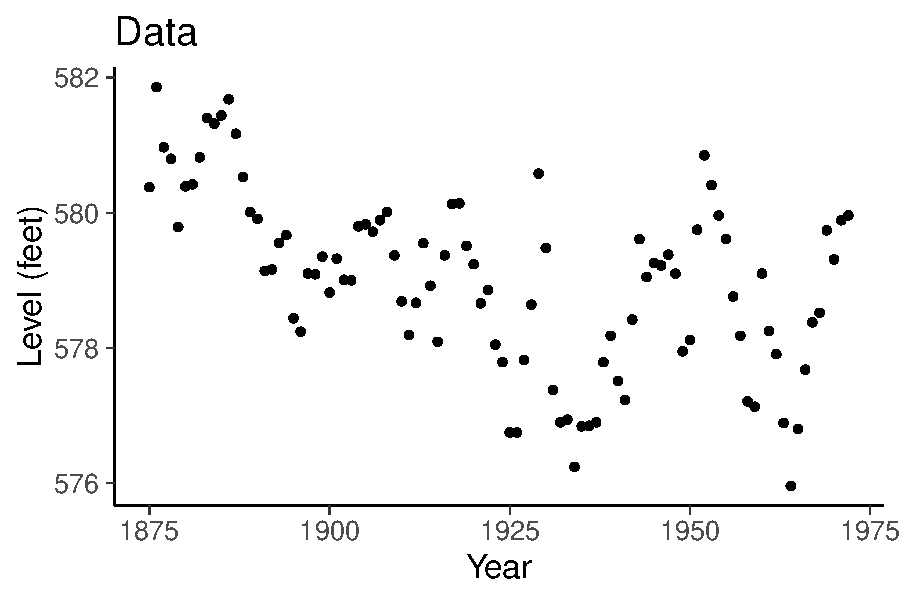
\includegraphics[width=10cm]{lake4data.pdf}}
  \only<2>{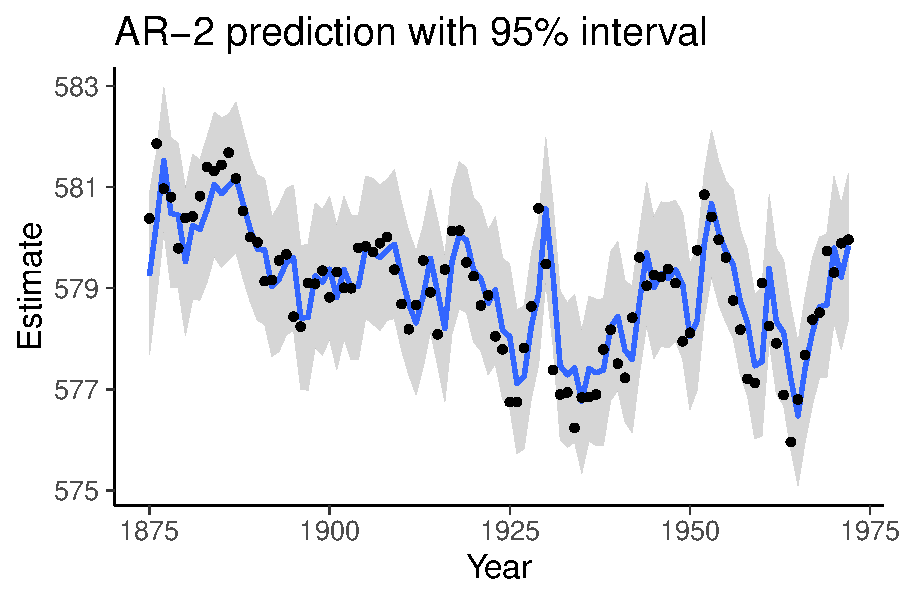
\includegraphics[width=10cm]{lake4pred.pdf}}
  \only<3>{\includegraphics[width=10cm]{lake4psismstep.pdf}}
  \only<4>{\includegraphics[width=10cm]{lake4psisrefits.pdf}}

  \vspace{3\baselineskip}
  \only<4> {\small \url{mc-stan.org/loo/articles/loo2-lfo.html}}

  
\end{frame}

\begin{frame}{}
  
{\Large\color{navyblue} K-fold cross-validation}

\begin{list1}
\item K-fold cross-validation can approximate LOO
  \begin{list2}
    \item all uses for LOO
  \end{list2}
\item K-fold cross-validation can be used for hierarchical models
  \begin{list2}
    \item good for leave-one-group-out
  \end{list2}
\item K-fold cross-validation can be used for time series
  \begin{list2}
    \item with leave-block-out
  \end{list2}
\end{list1}

\end{frame}

\begin{frame}{}

  \only<1>{\includegraphics[width=10cm]{lake3kfoldbal1.pdf}}
  \only<2>{\includegraphics[width=10cm]{lake3kfoldbal2.pdf}}
  \only<3>{\includegraphics[width=10cm]{lake3kfoldrand.pdf}}
  \only<4>{\includegraphics[width=10cm]{rats1kfoldrand.pdf}}
  \only<5->{\includegraphics[width=10cm]{rats1oneratb.pdf}}
  \\
  \only<6>{kfold\_split\_random()\\ \vspace{0.2\baselineskip}
  kfold\_split\_balanced()\\ \vspace{0.2\baselineskip}
  kfold\_split\_stratified()}
  
\end{frame}

\begin{frame}{}

{\Large\color{navyblue} WAIC vs PSIS-LOO}

\begin{list1}
  \item<2-> WAIC has same assumptions as LOO
  \item<3-> PSIS-LOO is more accurate 
  \item<4-> PSIS-LOO has much better diagnostics
  \item<5-> LOO makes the prediction assumption more clear,\\ which
    helps if K-fold-CV is needed instead
  \item<6-> Multiplying by -2 doesn't give any benefit\\ (Watanabe
    didn't multiply by -2)
\end{list1}

\vspace{6\baselineskip}
{\small see \href{http://link.springer.com/article/10.1007/s11222-016-9696-4}{Vehtari, Gelman \& Gabry (2017a)}}
\end{frame}

\begin{frame}{}

{\Large\color{navyblue} *IC}

\begin{list1}
  \item AIC uses maximum likelihood estimate for prediction
  \item DIC uses posterior mean for prediction
  \item BIC is an approximation for marginal likelihood
  \item TIC, NIC, RIC, PIC, BPIC, QIC, AICc, ...
\end{list1}

\end{frame}

\begin{frame}{}

{\Large\color{navyblue} Marginal likelihood / Bayes factor}

\vspace{-0.3\baselineskip}
\begin{list1}
\item Like leave-future-out 1-step-ahead corss-validation but starting with 0 observations\\
  \onslide<3->{- which makes it very sensitive to prior}
  \onslide<4->{and \\- unstable in case of misspecified
    models}\uncover<5->{ also asymptotically}
\end{list1}
\vspace{-0.5\baselineskip}
  \onslide<2->{\includegraphics[width=9.4cm]{lake3bf.pdf}}

\end{frame}

\begin{frame}{}

{\Large\color{navyblue} Cross-validation for model assessment}

\begin{list1}
\item CV is good for model assessment when application specific utility/cost functions are used
  \begin{list2}
  \item e.g. 90\% absolute error
  \end{list2}
\item<2-> Also useful in model checking in similar way as posterior
  predictive checking (PPC)
  \begin{list2}
  \item model misspecification diagnostics\\ (e.g. Pareto-$k$ and p\_loo)
  \item checking calibration of leave-one-out predictive posteriors
    (ppc\_loo\_pit in bayesplot)
  \end{list2}
  {\small see demos \url{avehtari.github.io/modelselection/}}
\end{list1}

\end{frame}

\begin{frame}
  
   {\Large\color{navyblue} Radon example}

   PSIS-LOO diagnostics
   \includegraphics[width=.8\textwidth]{radon1k.pdf}

{\small see \href{http://link.springer.com/article/10.1007/s11222-016-9696-4}{Vehtari, Gelman \& Gabry (2017a)}}
   
 \end{frame}


\begin{frame}
  
{\Large\color{navyblue} Sometimes cross-validation is not needed}

\vspace{-0.5\baselineskip}

  \begin{list1}
  \item<2-> Posterior predictive checking is often sufficient\\
    \vspace{0.5\baselineskip}
    \includegraphics[width=11cm]{mesquite_ppc.pdf}\\
  \vspace{-0.1\baselineskip} {Predicting the yields of mesquite bushes.\\
    \color{gray} \footnotesize
    Gelman, Hill \& Vehtari (2019): Regression and Other Stories, Chapter 11.}\\
  \vspace{-0.8\baselineskip}
\end{list1}
{\footnotesize
  \begin{list2}
  \item<3-> BDA3, Chapter 6
  \vspace{-0.6\parskip}
  \item<3-> Gabry, Simpson, Vehtari, Betancourt, Gelman
    (2018). Visualization in Bayesian workflow. JRSS A, \href{https://arxiv.org/abs/1709.01449}{preprint
      arXiv:1709.01449}
  \vspace{-0.6\parskip}
  \item<3-> \url{mc-stan.org/bayesplot/articles/graphical-ppcs.html}
  \vspace{-0.6\parskip}
  \item<3-> \url{betanalpha.github.io/assets/case_studies/principled_bayesian_workflow.html}
   \end{list2}}
\end{frame}

\begin{frame}{}

{\Large\color{navyblue} Model comparison}

\begin{list1}
\item ``A popular hypothesis has it that primates with larger brains
  produce more energetic milk, so that brains can grow quickly'' (from
  Statistical Rethinking)
  \begin{list2}
    \item Model 1: formula = kcal.per.g $\sim$ neocortex
    \item Model 2: formula = kcal.per.g $\sim$ neocortex + log(mass)
  \end{list2}
\end{list1}

\vspace{10\baselineskip}
{\small \url{mc-stan.org/loo/articles/loo2-example.html}}

\end{frame}

\begin{frame}

  \only<1-2>{\includegraphics[width=10cm]{milkelpdloo.pdf}}
  \only<3>{\includegraphics[width=10cm]{milkelpdloo2.pdf}}
  \\
  \only<2-3>{Model 1 elpd\_loo $\approx$ 3.7, SE=1.8\\
  Model 2 elpd\_loo $\approx$ 8.4, SE=2.8}

\end{frame}

\begin{frame}[fragile]

  {\includegraphics[width=10cm]{milkelpddiff.pdf}}
  \\
  {\scriptsize
\begin{lstlisting}
Model comparison: 
(negative 'elpd_diff' favors 1st model, positive favors 2nd) 

elpd_diff        se 
      4.7       2.7 
\end{lstlisting}}

\end{frame}

\begin{frame}

  {\Large\color{navyblue} Arsenic well example -- Model comparison}

   
   \includegraphics[width=.8\textwidth]{arsenic12d.pdf}

   An estimated difference in ${\rm elpd}_{\rm loo}$ of 16.4 with SE of 4.4.
   
{\small see \href{http://link.springer.com/article/10.1007/s11222-016-9696-4}{Vehtari, Gelman \& Gabry (2017a)}}
\end{frame}

\begin{frame}
  
{\Large\color{navyblue} Sometimes cross-validation is not needed}

\vspace{-0.5\baselineskip}

  \begin{list1}
  \item Posterior predictive checking is often sufficient\\
    \vspace{0.5\baselineskip}
    \includegraphics[width=11cm]{mesquite_ppc.pdf}\\
  \vspace{-0.1\baselineskip} {Predicting the yields of mesquite bushes.\\
    \color{gray} \footnotesize
    Gelman, Hill \& Vehtari (2019): Regression and Other Stories, Chapter 11.}\\
  \vspace{-0.8\baselineskip}
\end{list1}
{\footnotesize
  \begin{list2}
  \item BDA3, Chapter 6
  \vspace{-0.6\parskip}
  \item Gabry, Simpson, Vehtari, Betancourt, Gelman
    (2018). Visualization in Bayesian workflow. JRSS A, \href{https://arxiv.org/abs/1709.01449}{preprint
      arXiv:1709.01449}
  \vspace{-0.6\parskip}
  \item \url{mc-stan.org/bayesplot/articles/graphical-ppcs.html}
  \vspace{-0.6\parskip}
  \item \url{betanalpha.github.io/assets/case_studies/principled_bayesian_workflow.html}
   \end{list2}}
\end{frame}

\begin{frame}{}

{\Large\color{navyblue} Sometimes cross-validation is not needed}

\begin{list1}
\item<+-> For some very simple cases you may assume that true model
  is included in the list of models considered ($M$-closed)
  \begin{list2}
  \item<+-> see predictive model selection in $M$-closed case by
    San Martini and Spezzaferri (1984)
  \item<+-> but you should not force your design of experiment or
    analysis to stay in the simplified world
  \end{list2}
% \item<+-> For fully non-parametric models you may assume that true model
%   is included in the list of models considered ($M$-closed)
%   \begin{list2}
%   \item<+-> related to talk by Chris Holmes
%   \item<.-> see
%     \href{http://dx.doi.org/10.1214/12-SS102}{Vehtari \& Ojanen
%       (2012)} for earlier references
% \item<+-> posterior convergence rate can be slow for fully non-parametric models
% \end{list2}
\item<+-> In nested case, often easier and
  more accurate to analyse posterior distribution of more complex
  model directly \\
  {\small \url{avehtari.github.io/modelselection/betablockers.html}}
   % \begin{list2}
   %   \item<3-> need to do some model checking anyway
   % \end{list2}
\end{list1}

\end{frame}

\begin{frame}{}

  {\Large\color{navyblue} Sometimes predictive model comparison can be useful}

      \begin{minipage}[t]{0.45\linewidth}
        \begin{center}
          \includegraphics[width=5cm]{fitg2_xx_areas.pdf}\\
          Marginal posterior intervals
        \end{center} 
      \end{minipage}
      \pause
      \begin{minipage}[t]{0.45\linewidth}
        \begin{center}
          \includegraphics[width=5cm]{fitg2_xx_scatter.pdf}\\
          Joint posterior density
        \end{center} 
      \end{minipage}

            \begin{center}
      {\scriptsize rstanarm + bayesplot}
    \end{center}

    \pause
    {\small
      see also \href{https://avehtari.github.io/modelselection/collinear.html}{Collinear demo}
    }

\end{frame}

\begin{frame}{}

  {\Large\color{navyblue}  What if one is not clearly better than others?}

  \begin{list1}
  \item<2-> Continuous expansion including all models?
    \begin{list2}
    \item and then analyse the posterior distribution directly\\
        {\small \url{avehtari.github.io/modelselection/betablockers.html}}
      \item sparse priors like regularized horseshoe prior instead of variable selection\\
        {\small video, refs and demos at
          \url{avehtari.github.io/modelselection/}}
    \end{list2}
  \item<3-> Model averaging with BMA or Bayesian stacking?\\
    {\small \url{mc-stan.org/loo/articles/loo2-example.html}}
  \item<4-> In a nested case choose simpler if assuming some cost for
    extra parts?\\
    {\small \url{andrewgelman.com/2018/07/26/parsimonious-principle-vs-integration-uncertainties/}}
  \item<5-> In a nested case choose more complex if you want to take
    into account all the uncertainties.\\
    {\small \url{andrewgelman.com/2018/07/26/parsimonious-principle-vs-integration-uncertainties/}}
  \end{list1}

\end{frame}

\begin{frame}

  {\Large\color{navyblue} Model averaging}
  
  \begin{list1}
  \item<+-> Prefer continuous model expansion
  \item<+-> If needed integrate over the model space = model averaging
  \item<+-> Bayesian stacking may work better than BMA
    \begin{list2}
    \item \href{https://projecteuclid.org/euclid.ba/1516093227}{Yao, Vehtari, Simpson, \& Gelman (2018)}
    \end{list2}
  \end{list1}
  
\end{frame}

\begin{frame}{}

  {\Large\color{navyblue}  Cross-validation and model selection}

  \begin{list1}
  \item<1-> Cross-validation can be used for model selection if
    \begin{list2}
      \item small number of models
      \item the difference between models is clear
    \end{list2}
  \item<2-> Do not use cross-validation to choose from a large set of models
    \begin{list2}
    \item selection process leads to overfitting
    % \item you may use projection predictive approach
    % \item useful when correlating variables make the posterior
    %   distribution analysis difficult\\
    %   {\small video, refs and demos  at \url{avehtari.github.io/modelselection/}\\
    %   and \href{http://link.springer.com/article/10.1007/s11222-016-9649-y}{Piironen \& Vehtari (2017)}}
    \end{list2}
  \item<3-> Overfitting in selection process is not unique for cross-validation
  \end{list1}
\end{frame}

\begin{frame}
  
  {\Large\color{navyblue} Selection induced bias and overfitting}

  \begin{itemize}
  \item Selection induced bias in cross-validation
    \begin{itemize}
    \item same data is used to assess the performance and make the selection
    \item the selected model fits more to the data
    \item the CV estimate for the selected model is biased
    \item recognised already, e.g., by Stone (1974)
    \end{itemize}
    \pause
  \item Performance of the selection process itself can be assessed
    using two level cross-validation, but it does not help choosing
    better models
    \pause
  \item Bigger problem if there is a large number of models as in
    covariate selection
  \end{itemize}

\end{frame}

\begin{frame}

  {\Large\color{navyblue} Selection induced bias in variable selection}

  \includegraphics[width=\textwidth]{cv.pdf}

\end{frame}

\begin{frame}

  {\Large\color{navyblue} Selection induced bias in variable selection}

  \includegraphics[height=0.88\textheight]{simulated_searchpath.pdf}
   \vspace{-1.5\baselineskip}
   \mbox{{\hspace{8cm} \footnotesize \href{http://link.springer.com/article/10.1007/s11222-016-9649-y}{Piironen \& Vehtari (2017)}}}

\end{frame}

\begin{frame}

  {\Large\color{navyblue} Selection induced bias in variable selection}

  \includegraphics[height=0.88\textheight]{simulated_variability.pdf}
   \vspace{-1.5\baselineskip}
   \mbox{{\hspace{8cm} \footnotesize \href{http://link.springer.com/article/10.1007/s11222-016-9649-y}{Piironen \& Vehtari (2017)}}}

\end{frame}

\begin{frame}

  {\Large\color{navyblue} Selection induced bias in variable selection}

  \includegraphics[height=0.88\textheight]{real_searchpath.pdf}
   \vspace{-2\baselineskip}
   \mbox{{\hspace{9.5cm} \parbox[t]{12cm}{\footnotesize \href{http://link.springer.com/article/10.1007/s11222-016-9649-y}{Piironen \&\\ Vehtari (2017)}}}}

\end{frame}


\begin{frame}{}

  {\Large\color{navyblue}  Take-home messages}

  \begin{list1}
  \item It's good to think predictions of observables, because
    observables are the only ones we can observe
  \item \only<1>{\color{gray}}Cross-validation can simulate predicting and observing new
    data
  \item \only<2>{\color{gray}}Cross-validation is good if you don't
    trust your model
  \item \only<3>{\color{gray}}Different variants of cross-validation
    are useful in different scenarios
  \item \only<4>{\color{gray}}Cross-validation has high variance, and
    {\bf if} you trust your model you can beat cross-validation in
    accuracy
  \end{list1}
  \only<5>{~}

\end{frame}

\end{document}

\begin{frame}

{\Large\color{navyblue} Bayesian stacking}

  \begin{itemize}
  \item Consider the model averaging as a decision problem with aim of
    maximizing the predictive performance
  \item<2-> Maximize the scoring rule of the predictive distribution for future $\tilde{y}$
    \begin{align*} \label{stacking_population}
      \max_{w}  S\Bigl(   \sum_{k=1}^K w_k p(\tilde{y} | x, y, M_k), p_t(\tilde{y}) \Bigr),  
    \end{align*}
  \item<3-> As we don't know $p_t(\tilde{y})$, we approximate with LOO
  \item<4-> We define the stacking weights as the solution to the following optimization problem:
\begin{align*} 
 \max_w \frac{1}{n}\sum_{i=1}^n S\Bigl( \sum_{k=1}^K  w_k \hat p(y_i|x_{-i},y_{-i},M_k) \Bigr) ,\\ \quad  s.t. \quad w_k \geq 0,   \quad \sum_{k=1}^K w_k=1.
\end{align*}
  \end{itemize}

\end{frame}

\begin{frame}

{\Large\color{navyblue} Bayesian stacking}

  \begin{itemize}
\item The combined estimation of the predictive density is
 \begin{align*} 
  \hat p(\tilde{y} |x, y)= \sum_{k=1}^K \hat{w}_k p(\tilde{y}|x, y, M_k).
  \end{align*}
\item<2-> When using log-score (corresponding to Kullback-Leibler
  divergence), we call this \emph{stacking of predictive
    distributions}:
\begin{align*}
  \max_w \frac{1}{n} \sum_{i=1}^n \log \sum_{k=1}^K w_k p(y_i | x_{-i}, y_{-i}, M_k) , \\
  \quad s.t.   \quad w_k \geq 0,   \quad \sum_{k=1}^K w_k=1.
\end{align*}
  \item<3-> We can approximate $p(y_i | x_{-i}, y_{-i}, M_k)$ with PSIS-LOO
  \item<4-> Other cross-validation structures can be used, too
  \end{itemize}
\end{frame}

\begin{frame}

{\Large\color{navyblue} Gaussian mixture example}

$y \sim \N(3.4, 1), \quad p_k = \N(k, 1) \text{ with } k = 1,\ldots,8$
\pause

Model averaged predictive distributions
 \includegraphics[width=12cm]{dis34.pdf}

\end{frame}

\begin{frame}

{\Large\color{navyblue} Gaussian mixture example}

$y \sim \N(3.4, 1), \quad p_k = \N(k, 1) \text{ with } k = 1,\ldots,8$

(a, b) {\color{red} Stacking of predictive distributions} vs. {\color{greenish} BMA}\\
  \vspace{0.2cm}

   \makebox[12cm][t]{
  \hspace{-0.7cm}
\begin{overlayarea}{12cm}{4.5cm}
 \includegraphics[width=12cm]{score34.pdf}\\
 \only<1>{\hide[white]{-0.4}{0.65}{0.4}{0.33}} %
\end{overlayarea}
}

\uncover<2->{
(c) Dilutation of prior by adding copies of $\N(4,1)$ to the model space
}

\end{frame}

\begin{frame}

{\Large\color{navyblue} Linear subset regression example $k$}

\vspace{-0.4\baselineskip}
$y \sim \N(\mu, 1), \quad \mu = \beta_1 X_1 + \ldots \beta_{15} X_{15}$\\
\only<1>{\makebox[12cm][t]{\scriptsize
$ \beta_j=\gamma\left(     (1_{ | j-4 | <h}  (h- |j-4|)^2  +(  1_{|j-8|<h }   )  (  h- |j-8|  )^2+ (   1_{|j-12|<h}    ) (  h-|j-12|  )^2 \right)$
}}

\pause
Non-nested $M$-open case with $M_k: \N(\beta_k X_k, \sigma)$\\ \pause
\vspace{-\baselineskip}
\makebox[12cm][t]{
  \hspace{-0.7cm}
\includegraphics[width=10.4cm]{single_variable_regression.pdf}
}\\
\vspace{-0.5\baselineskip}
(a) {\color{red}Stacking}, (b) {\color{red}BMA},
(d) model selection by {\color{red}LOO} and {\color{blue}BF}\\
{\vspace{-5.5cm}\hspace{2.4cm}(a)}{\hspace{4.2cm}(b)}\\
{\vspace{2.5cm}\hspace{7.1cm}(d)}

\end{frame}

\begin{frame}

{\Large\color{navyblue} Linear subset regression example $1:k$}

\vspace{-0.4\baselineskip}
$y \sim \N(\mu, 1), \quad \mu = \beta_1 X_1 + \ldots \beta_{15} X_{15}$\\
Nested $M$-closed case with $M_k: \N( \sum_{j=1}^k \beta_j X_j, \sigma)$\\ \pause
\vspace{-\baselineskip}
\makebox[12cm][t]{
  \hspace{-0.7cm}
  \includegraphics[width=10.4cm]{linear_regression.pdf}
}\\
\vspace{-0.5\baselineskip}
(a) {\color{red}Stacking}, (b) {\color{red}BMA},
(d) model selection by {\color{red}LOO} and {\color{blue}BF}\\
{\vspace{-5.5cm}\hspace{2.4cm}(a)}{\hspace{4.2cm}(b)}\\
{\vspace{2.5cm}\hspace{7.1cm}(d)}


\end{frame}

\begin{frame}

{\Large\color{navyblue} Variational multimodal example}

Stacking of predictive distributions can be helpful also in case of
multimodal posteriors\\
\vspace{-\baselineskip}
\makebox[12cm][t]{
  \hspace{-0.7cm}
  \includegraphics[width=12.5cm]{vb.pdf}
}

\end{frame}

%\begin{frame}

% {\Large\color{navyblue} Non-linear model example}

%   \begin{center}
%   \includegraphics[width=\textwidth]{wells.pdf}
%   \end{center}

% \end{frame}

% \begin{frame}

% {\Large\color{navyblue} Non-linear model example}

%   \begin{center}
%   \includegraphics[width=\textwidth]{wells_combine.pdf}
%   \end{center}

% \end{frame}

\begin{frame}

{\Large\color{navyblue} Bayesian stacking}
  
  \begin{itemize}
  \item In $M$-open case works better than BMA
  \item In $M$-closed case can have a better small sample performance than BMA
  \item<2-> Should be used only for model averaging
    \begin{list2}
    \item you may drop models with 0 weights
    \item you shouldn't choose the model with largest weight unless it's 1
    \end{list2}
  \item<2-> \href{https://projecteuclid.org/euclid.ba/1516093227}{Yao, Vehtari, Simpson, \& Gelman (2018)}
  \end{itemize}
  
\end{frame}


\begin{frame}{}

  {\Large\color{navyblue} Part 2: Projective Inference in
    High-dimensional Problems: Prediction and Feature
    Selection}

\end{frame}

\begin{frame}{}

  {\Large\color{navyblue} High dimensional small data}

  \begin{itemize}
  \item In the examples $n = 54...102$, $p=1536...22283$
    \begin{itemize}
    \item could scale to bigger $n$ and bigger $p$
    \end{itemize}
  \item<2-> Priors necessary
    \begin{itemize}
    \item shrinkage priors, hierarchical shrinkage priors
    \item dimension reduction with factor models
    \end{itemize}
    \vspace{\baselineskip}
  \item<3-> The main content of this part: Two stage approach
    \begin{itemize}
    \item Construct a best predictive model you can\\ $\Rightarrow$ {\it reference model}
    \item Feature selection and post-selection inference\\ $\Rightarrow$ {\it projection}
    \end{itemize}
  \end{itemize}
  
\end{frame}

\begin{frame}{}

  {\Large\color{navyblue} Rich model vs feature selection?}

  \begin{itemize}
  \item If we care only about the predictive performance
    \begin{itemize}
    \item Include all available prior information
    \item Integrate over all uncertainties
    \item No need for feature selection
    \end{itemize}
  \item<2-> Variable selection can be useful if
    \begin{itemize}
    \item need to reduce measurement or computation cost in the future
    \item improve explainability
    \end{itemize}
  \item<3-> Two options for variable selection
    \begin{itemize}
    \item Find a minimal subset of features that yield a good
      predictive model
    \item Identify all features that have predictive information
    \end{itemize}
  \end{itemize}
  
\end{frame}

\begin{frame}{}

  {\Large\color{navyblue} Regularized horseshoe prior}
  
  \vspace{-0.3\baselineskip}
  \begin{itemize}
  \item Horseshoe: can be seen as continuos version of spike-and-slab with
    {\it infinite} width slab
    \begin{itemize}
    \item no shrinkage ($\kappa_j \rightarrow 0$) allows complete separation in logistic model with $n \ll p$\\
      \vspace{0.5\baselineskip}
      \includegraphics[width=5.5cm]{hs_vs_spikeandslab.png}
    \end{itemize}
    % \vspace{0.5\baselineskip}
  \item<2-> Regularized horseshoe: adds additional {\it finite} width slab
    \begin{itemize}
    \item some minimal shrinkage ($\kappa_j > 0$) for relevant features, but maintains division to relevant and non-relevant features\\
      \vspace{0.5\baselineskip}
      \includegraphics[width=5.5cm]{rhs_vs_spikeandslab.png}
    \end{itemize}
  \end{itemize}
\end{frame}

\begin{frame}

  {\Large\color{navyblue} Regularized horseshoe}

  \begin{itemize}
    \item {\small Piironen and Vehtari (2017). Sparsity information and
      regularization in the horseshoe and other shrinkage priors. In
      Electronic Journal of Statistics, 11(2):5018-5051. \href{https://projecteuclid.org/euclid.ejs/1513306866}{Online}}
      \begin{itemize}
      \item regularized horseshoe
      \item how to set the prior based on the sparsity assumption
      \end{itemize}
  \end{itemize}

\end{frame}

\begin{frame}{}

  {\Large\color{navyblue} Why shrinkage priors alone do not solve the
    variable selection problem}

  \begin{itemize}
  \item A common strategy:
    \begin{itemize}
    \item Fit model with a shrinkage prior
    \item Select variables based on marginal posteriors (of the
      regression coefficients)
    \end{itemize}
  \item<2-> Problems
    \begin{itemize}
    \item Marginal posteriors are difficult with correlated features
    \item How to do post-selection inference correctly?
    \end{itemize}
  \end{itemize}
\end{frame}

\begin{frame}{}

  {\Large\color{navyblue} Example}

Consider data
\begin{equation*}
  \color{gray}
\begin{alignedat}{2}
  \only<1>{\color{black}}f & \only<1>{\color{black}} \sim \N(0,1), &&  \\
  \only<2>{\color{black}}y \mid f &\only<2>{\color{black}}\sim \N(f, 1) && \\
  \only<3>{\color{black}}x_j \mid f &\only<3>{\color{black}}\sim \N(\sqrt{\rho}f,\, 1-\rho), \qquad &&\only<3>{\color{black}} j = 1,\dots,25 \,, \\
  \only<4>{\color{black}}x_j \mid f &\only<4>{\color{black}}\sim \N(0, 1), && \only<4>{\color{black}}j = 26,\dots, 50 \,.
\end{alignedat}
\end{equation*}

\begin{itemize}
\item<2-> $y$ are noisy observations about latent $f$ \pause
\item<3-> First $p_\text{rel}=25$ features are correlated with $\rho$ and predictive about $y$ \pause
\item<4-> Remaining $25$ features are irrelevant random noise
\end{itemize}
\uncover<5>{Generate one data set $\{ x^{(i)}, y^{(i)}\}^n_{i=1}$ with $n=50$ and $\rho=0.8$ and assess the feature relevances}

\end{frame}

\begin{frame}{}

  {\Large\color{navyblue} Example}

  \makebox[12.1cm][t]{
    \hspace{-0.9cm}
  \begin{minipage}[b][4cm][t]{12.1cm}
  \includegraphics[width=4cm]{toy_marginal1.pdf}
  \uncover<2->{\includegraphics[width=4cm]{toy_marginal2.pdf}}
  \uncover<3->{\includegraphics[width=4cm]{toy_marginal3.pdf}}\\
\end{minipage}
}\\
\uncover<1->{
	A) Gaussian prior, posterior median with 50\% and 90\% intervals\\ 
	}
	\uncover<2->{
	B) Horseshoe prior, same things\\ 
	}
	\uncover<3->{
	C) Spike-and-slab prior, posterior inclusion probabilities\\ 
      }
      ~\\
      \uncover<4>{Half of the features relevant, but all marginals
        substantially overlapping with zero}
\end{frame}

\begin{frame}{}

  {\Large\color{navyblue} What happens?}

  \makebox[12.1cm][t]{
    \hspace{-0.3cm}
    \begin{minipage}[b][8.1cm][t]{12.1cm}
      \makebox[0cm][t]{\hspace{-0.4cm}\rotatebox{90}{\hspace{1.4cm}Gaussian}}
      \includegraphics[width=3.7cm]{toy_scatter1.pdf}
      \uncover<2->{\includegraphics[width=3.7cm]{toy_scatter3.pdf}}
      \uncover<3->{\includegraphics[width=3.7cm]{toy_scatter5.pdf}}\\
      \makebox[0cm][t]{\hspace{-0.4cm}\rotatebox{90}{\hspace{1.4cm}Horseshoe}}
      \includegraphics[width=3.7cm]{toy_scatter2.pdf}
      \uncover<2->{\includegraphics[width=3.7cm]{toy_scatter4.pdf}}
      \uncover<3->{\includegraphics[width=3.7cm]{toy_scatter6.pdf}}\\
      \makebox[3.7cm]{$\quad p_\text{rel}=2$}
      \uncover<2->{\makebox[3.7cm]{$\quad p_\text{rel}=5$}}
      \uncover<3->{\makebox[3.7cm]{$\quad p_\text{rel}=25$}}
\end{minipage}
}
\end{frame}

\begin{frame}{}

  {\Large\color{navyblue} Focus on predictive performance}

  \begin{itemize}
  \item Two stage approach
    \begin{itemize}
    \item Construct a best predictive model you can\\ $\Rightarrow$ {\it reference model}
    \item Variable selection and post-selection inference\\ $\Rightarrow$ {\it projection}
    \end{itemize}
  \item<2-> Instead of looking at the marginals, find the minimal
    subset of features which have (almost) the same predictive
    performance as the reference model
  \end{itemize}
  
\end{frame}

\begin{frame}{}

  {\Large\color{navyblue} Reference model improves variable selection}

  Same data generating mechanism, but\\ $n=30$, $p=500$, $p_\text{rel}=150$, $\rho=0.5$.

  \includegraphics[width=5.5cm]{toy_corr1.pdf}\\
  \vspace{-0.2cm}
  \hspace{0.5cm} {\color{set12} irrelevant $x_j$}, {\color{set11} relevant $x_j$}\\
  \vspace{0.2cm}
  \hspace{0.5cm} Sample correlation with $y$\\
  
\end{frame}

\begin{frame}{}

  {\Large\color{navyblue} Reference model improves variable selection}

  \includegraphics[width=5.5cm]{toy_corr2.pdf}
  \uncover<2->{\includegraphics[width=5.5cm]{toy_corr3.pdf}}\\
  \vspace{-0.2cm}
  \hspace{0.5cm} {\color{set12} irrelevant $x_j$}, {\color{set11} relevant $x_j$}\\
  \vspace{0.2cm}
  A) Sample correlation with $y$ vs. sample correlation with $f$\\
  \uncover<2->{B) Sample correlation with $y$ vs. sample correlation with $f_*$\\
  $f_* = $ linear regression fit with 3 supervised principal components}
  
\end{frame}

\begin{frame}{}

  {\Large\color{navyblue} (Iterative) Supervised Principal Components}

  \begin{itemize}
  \item Dimension reduction for high dimensional small data with
    highly correlating features
    \begin{itemize}
    \item dimension reduction helps to speed up later computation
      without discarding much information
    \item supervised means that features correlating with the target
      are favored in construcing the principal components
    \end{itemize}
    {\small
    \item     Piironen and Vehtari (2018). Iterative supervised principal components. 21st AISTATS, PMLR 84:106-114. \href{http://proceedings.mlr.press/v84/piironen18a.html}{Online}.
    }
  \end{itemize}
  
\end{frame}

\begin{frame}{}

  {\Large\color{navyblue} Predictive projection, idea}
  
  \begin{itemize}
  \item Model simplification technique
  \item<2-> Replace full posterior $p(\theta \mid D)$ with
    some constrained $q(\theta)$ so that the \emph{predictive
      distribution} changes as little as possible
  \item<3-> Example constraints
    \begin{itemize}
    \item $q(\theta)$ can have only point mass at some $\theta_0$ \\
      $\Rightarrow$ ``Optimal point estimates''
    \item<4-> Some features must have exactly zero regression coefficient \\
      $\Rightarrow$ ``Which features can be discarded''
    \end{itemize}
    \vspace{1\baselineskip}
  \item<5-> The decision theoretic idea of conditioning the smaller
    model inference on the full model can be tracked to Lindley (1968)
    \begin{itemize}
    \item draw by draw projection introduced by Goutis \& Robert
      (1998), and Dupuis \& Robert (2003)
    \item see also many related references in a review by
      \href{http://dx.doi.org/10.1214/12-SS102}{Vehtari \& Ojanen
        (2012)}
    \end{itemize}
\end{itemize}

\end{frame}

\begin{frame}{}

  {\Large\color{navyblue} Logistic regression with two features}

  \vspace{\baselineskip}
  
  \begin{overlayarea}{\textwidth}{0.7\textwidth}
    \begin{minipage}{0.99\textwidth}
      \begin{center}
        \only<1>{ \minput{proj_posterior} }%
        \only<2>{ \minput{proj_b1b2_single} }%
        \only<3>{ \minput{proj_b2_single} }%
        \only<4>{ \minput{proj_b1_single} }%
        \only<5>{ \minput{proj_b2_dbd} }%
        \only<6>{ \minput{proj_b1_dbd} }%
      \end{center}
    \end{minipage}
    \begin{minipage}{0.99\textwidth}
      \only<1>{Full posterior for $\beta_1$ and $\beta_2$ and contours of predicted class probability}
      \only<2>{Projected point estimates for $\beta_1$ and $\beta_2$}
      \only<3>{Projected point estimates, constraint $\beta_1 = 0$}
      \only<4>{Projected point estimates, constraint $\beta_2 = 0$}
      \only<5>{Draw-by-draw projection, constraint $\beta_1 = 0$}
      \only<6>{Draw-by-draw projection, constraint $\beta_2 = 0$}
    \end{minipage}
  \end{overlayarea}
\end{frame}

\begin{frame}

  {\Large\color{navyblue} Predictive projection}


  \begin{itemize}
  \item Replace full posterior $p(\theta \mid D)$ with some
    constrained $q(\theta)$ so that the \emph{predictive distribution}
    changes as little as possible
  \item<2-> As the full posterior $p(\theta \mid D)$ is projected to $q(\theta)$
    \begin{itemize}
    \item the prior is also projected and there is no need to define
      priors for submodels separately
    \item<3-> even if we constrain some coefficients to be $0$, the
      predictive inference is conditoned on the information related
      features contributed to the reference model
    \end{itemize}
  \end{itemize}

  
\end{frame}

\frame{

  {\Large\color{navyblue} Projective selection}

\begin{itemize}
	\item How to select a feature combination? \pause
	\item For a given model size, choose feature combination with minimal projective loss \pause
	\item Search heuristics, e.g. 
	\begin{itemize}
        \item Monte Carlo search
        \item Forward search
        \item $L_1$-penalization (as in Lasso)
	\end{itemize} \pause 
      \item Use cross-validation to select the appropriate model size
        \begin{itemize}
        \item need to cross-validate over the search paths
        \end{itemize}
      \end{itemize} 
}

\frame{

  {\Large\color{navyblue} Projective selection vs. Lasso}

Same simulated regression data as before, \\ 
$n=50$, $p=500$, $p_\text{rel} = 150$, $\rho=0.5$

\vspace{0.5em}

  \makebox[12.1cm][t]{
    \hspace{-0.5cm}
  \begin{minipage}{0.99\textwidth}
      \only<1>{\includegraphics[width=5.5cm]{vslasso1rmse.pdf}}
      \only<2>{\includegraphics[width=5.5cm]{vslasso2rmse.pdf}}
      \only<3->{\includegraphics[width=5.5cm]{vslasso3rmse.pdf}}
      \uncover<4>{\includegraphics[width=5.5cm]{vslasso3mlpd.pdf}}
  \end{minipage}
  }
  
}

\frame{

  {\Large\color{navyblue} Real data benchmarks}\\
  $n = 54...102$, $p=1536...22283$, Bayes SPC as the reference
\begin{overlayarea}{\textwidth}{0.7\textwidth}
\vspace{-0.5em}
	\begin{minipage}{0.99\textwidth}
	\begin{center}
          \minput[pdf]{realdata}
	\end{center}
	% hidings
	\only<1>{ \hide[white]{-0.5}{-0.02}{0.42}{1.05} }%
	\only<2>{ \hide[white]{-0.3}{-0.02}{0.22}{1.05} }%
	\only<3>{ \hide[white]{-0.07}{-0.02}{0.01}{1.05} }%
	
	\end{minipage}
	%\begin{minipage}{0.99\textwidth}
	%\end{minipage}
	
\end{overlayarea}
}

\frame{

  {\Large\color{navyblue} Computation time}

  \begin{table}%
    \small
\vspace{-0.2cm}
\centering
\abovetopsep=2pt
\begin{tabular}{ lccrrrr }
\toprule
Data set & $n$ & $p$ & \multicolumn{4}{c}{Computation time} \\
\cmidrule(r){4-7}
 & & & Bayes SPC & Projection & Lasso1 & Lasso2 \\ 
\midrule
Ovarian & 54 & 1536 & 30.4 & 3.6 & 1.3 & 0.2  \\
Colon & 62 & 2000 & 31.0 & 4.0 & 1.6 & 0.3  \\
Prostate & 102 & 5966 & 49.4 & 7.6 & 5.0 & 0.8 \\
Leukemia & 72 & 7129 & 47.0 & 6.3 & 5.6 & 0.7  \\
Glioma & 85 & 22283 & 95.8 & 14.2 & 15.6 & 2.6 \\
\bottomrule
\end{tabular}
\caption{{\it Computation times:} Average computation time (in seconds) over five repeated runs. In all cases the time contains the cross-validation of the tuning parameters and/or the model size. The first result for Lasso is computed using our software ({\tt projpred}) whereas the second result (and that of ridge) is computed using the R-package {\tt glmnet} which is more highly optimized. }
\label{tab:computation_times}
\end{table}
}

\begin{frame}

  {\Large\color{navyblue} Selection induced bias in variable selection}

  \includegraphics[height=0.88\textheight]{simulated_variability.pdf}
   \vspace{-1.5\baselineskip}
   \mbox{{\hspace{8cm} \footnotesize \href{http://link.springer.com/article/10.1007/s11222-016-9649-y}{Piironen \& Vehtari (2017)}}}

\end{frame}

\begin{frame}

  {\Large\color{navyblue} Selection induced bias in variable selection}

  \includegraphics[height=0.88\textheight]{real_searchpath.pdf}
   \vspace{-2\baselineskip}
   \mbox{{\hspace{9.5cm} \parbox[t]{12cm}{\footnotesize \href{http://link.springer.com/article/10.1007/s11222-016-9649-y}{Piironen \&\\ Vehtari (2017)}}}}

\end{frame}

\begin{frame}
  
  {\Large\color{navyblue} Bodyfat: small $p$ example of projection predictive}
  
  Predict bodyfat percentage. The reference value is obtained by
  immersing person in water. $n=251$.

  \pause
  \vspace{-0.7\baselineskip}
  \includegraphics[width=7.7cm]{bodyfat_corr.pdf}

\end{frame}

\begin{frame}
  
  {\Large\color{navyblue} Bodyfat}

  Marginal posteriors of coefficients
  
  \includegraphics[width=11cm]{bodyfat_mcmc_areas.pdf}

\end{frame}

\begin{frame}
  
  {\Large\color{navyblue} Bodyfat}

  Bivariate marginal of weight and height
  
  \includegraphics[width=7.5cm]{bodyfat_mcmc_scatter.pdf}

\end{frame}

\begin{frame}
  
  {\Large\color{navyblue} Bodyfat}

  The predictive performance of the full and submodels
  
  \includegraphics[width=11cm]{bodyfat_varsel_plot.pdf}

\end{frame}


\begin{frame}
  
  {\Large\color{navyblue} Bodyfat}

  Marginals of projected posterior
  
  \includegraphics[width=11cm]{bodyfat_proj_mcmc_areas.pdf}

\end{frame}

\begin{frame}
  
  {\Large\color{navyblue} Bodyfat}

  Projected posterior is not just the conditional of joint
  
  \includegraphics[width=7.5cm]{bodyfat_proj_mcmc_scatter.pdf}

\end{frame}


\begin{frame}
  
  {\Large\color{navyblue} Bodyfat}

  Projected posterior is different than posterior conditioned only on selected features

  \vspace{-0.7\baselineskip}
  \includegraphics[width=11cm]{bodyfat_compare_sigmas.pdf}

\end{frame}

% Case study \url{avehtari.github.io/modelselection/bodyfat.html}
\begin{frame}
  
  {\Large\color{navyblue} Projection of Gaussian graphical models}\\

  \begin{itemize}
  \item Williams, Piironen, Vehtari, Rast (2018). Bayesian estimation of Gaussian graphical models with projection predictive selection. \href{https://arxiv.org/abs/1801.05725}{arXiv:1801.05725}\\
    \includegraphics[width=8.5cm]{ceu.pdf}\\
    {\footnotesize CEU genetic network. BGL: Bayesian glasso; GL: glasso;
      TIGER: tuning insensitive graph estimation and regression; BMA:
      Bayesian model averaging; MAP: Maximum a posteriori; Projection:
      projection predictive selection.}
  \end{itemize}
  
\end{frame}

\begin{frame}
  
  {\Large\color{navyblue} More results}\\

  {\footnotesize
  \begin{itemize}
  \item More results projpred vs. Lasso and elastic net:\\
    Piironen, Paasiniemi, Vehtari (2018). Projective Inference in
    High-dimensional Problems: Prediction and Feature Selection.
    \href{https://arxiv.org/abs/arXiv:1810.02406}{arXiv:1810.02406}
  \item More results projpred vs. marginal posterior probabilities:\\
    Piironen and Vehtari (2017). Comparison of Bayesian predictive
    methods for model selection. Statistics and Computing,
    27(3):711-735.
    \href{https://dx.doi.org/10.1007/s11222-016-9649-y}{doi:10.1007/s11222-016-9649-y}.
  \item projpred for Gaussian graphical models:\\
    Williams, Piironen, Vehtari, Rast (2018). Bayesian estimation of Gaussian graphical models with projection predictive selection. \href{https://arxiv.org/abs/1801.05725}{arXiv:1801.05725}
  \item More results for Bayes SPC:\\
    Piironen and Vehtari (2018). Iterative supervised principal components. 21st AISTATS, PMLR 84:106-114. \href{http://proceedings.mlr.press/v84/piironen18a.html}{Online}.
  \item Several case studies for small to moderate dimensional ($p=4 \ldots 100$) small data:\\
    Vehtari (2018). Model assesment, selection and inference after
    selection. \url{https://avehtari.github.io/modelselection/}
  \end{itemize}
  }
\end{frame}


\frame{

  {\Large\color{navyblue} Take-home messages (part 2)}

\begin{itemize}
\item Sparse priors do not automate variable selection
  \begin{itemize}
  \item Don't trust marginal posteriors
  \end{itemize}
\item<2-> Reference model + projection can improve feature selection
  \begin{itemize}
  \item Excellent tradeoff between accuracy and model complexity
  \item Useful also for identifying all the relevant features
  \end{itemize}
\item<3-> Well developed for GLMs, but can be used also with other model families
\item<4-> More details and results (+ some theoretical discussion) in the paper
  \begin{itemize}
  \item Piironen, Paasiniemi, Vehtari (2018). Projective Inference in
    High-dimensional Problems: Prediction and Feature
    Selection. \href{https://arxiv.org/abs/arXiv:1810.02406}{arXiv:1810.02406}
  \end{itemize}
\item<5-> R-package {\tt projpred} in CRAN and github
  \url{https://github.com/stan-dev/projpred}\\ (easy to use, e.g. with
  RStan, RStanARM, brms)
\end{itemize}
}

\begin{frame}{}

  {\Large\color{navyblue}  References}

  References and more at \url{avehtari.github.io/masterclass/} and
  \url{avehtari.github.io/modelselection//}
  \begin{list1}
  \item Model selection tutorial at StanCon 2018 Asilomar
    \begin{list2}
    \item more about projection predictive variable selection
    \end{list2}
  \item Regularized horseshoe talk at StanCon 2018 Asilomar
  \item Several case studies
  \item References with links to open access pdfs
  \end{list1}
  
\end{frame}

\end{document}

%%% Local Variables: 
%%% mode: latex
%%% TeX-master: t
%%% End:
